\documentclass[a4paper,11pt,twoside,pdftex]{article}
%\DeclareGraphicsExtensions{.pdf,.gif,.jpg} %this tells latex what kinds of files to expect for your figures
% Caption package for formating figure and label captions
\usepackage[font=bf,format=hang,labelsep=colon,justification=justified,singlelinecheck=false,compatibility=false]{caption}

% Misc packages
\usepackage{ifthen} % for conditional expressions
\usepackage{float} % for floating tables and graphics
\usepackage{setspace} % for defining spacing between lines
\usepackage{cmap} % allow searching in pdf documents
\usepackage{tabulary} % better tables
\usepackage{comment} % block comments
\usepackage{multicol}
\usepackage[toc,page]{appendix}
\usepackage{subfig}
\usepackage{amsfonts}

\usepackage[normalem]{ulem}
\usepackage{url}
\usepackage{bm}
%\usepackage[usenames, dvipsnames]{color} % Highlighting text for editing


%%%%%%%%%%%%%%%%
%% distributions
%%%%%%%%%%%%%%%%
\newcommand{\distn}{\mathcal{N}}  %% Normal distribution
\newcommand{\distln}{\mathcal{LN}}  %% Lognormal distribution
\newcommand{\distbern}{\mathcal{B}ern}  %% Bernoulli distribution
\newcommand{\distmulti}{\mathcal{M}ultinomial}
%%%%%%%%%%%%%%%%
%% Indexes
%%%%%%%%%%%%%%%%
\newcommand{\tagnd}{k}
\newcommand{\timend}{t}
\newcommand{\yearnd}{y}
\newcommand{\agend}{a}
\newcommand{\lennd}{l}
\newcommand{\regnd}{c}
\newcommand{\agent}{i}
% hyperref for HTML links within pdf 
%% EXAMPLE: \href{http://www.niwa.co.nz}{NIWA}
\usepackage[bookmarks=true,bookmarksopen=false,bookmarksnumbered=true,
            pdfpagelayout=TwoPageRight,
            pdftitle={IBM User Manual (Beta Version)}, 
            pdfauthor={C. Marsh} %authors
            pdfsubject={IBM, User manual},
            pdftex]{hyperref}
\hypersetup{
  breaklinks=true,      % allow line breaks in URLs
  colorlinks=true,      % use colour to define links
  linkcolor=black,      % colour of internal links
  citecolor=black,      % colour of links to bibliography
  filecolor=black,      % colour of file links
  urlcolor=darkgray     % colour of external links
}
\pdfadjustspacing=1

% Use AMS Maths 
\usepackage[fleqn]{amsmath}
\newcommand\AddVspace{\\[0 pt]} % artificial method of adding vertical space within equations

% Package for including and pretty printing of external config files and program code
\usepackage{listings} 
\lstset{ %
basicstyle=\ttfamily\footnotesize,
breaklines=true,
columns=fullflexible,
showspaces=false,               % show spaces adding particular underscores
showstringspaces=false,         % underline spaces within strings
showtabs=false,                 % show tabs within strings adding particular underscores
tabsize=2,			            % sets default tabsize to 2 spaces
breakatwhitespace=false,	    % sets if automatic breaks should only happen at whitespace
escapeinside={\%*}{*)}          % if you want to add a comment within your code
}

% highlighting package for editing
\usepackage{color,soul}

% Allow colour for HTML links
\usepackage{color}
\definecolor{darkgray}{gray}{0.20}
\definecolor{lightgray}{gray}{0.95}

% Geometery for A4 layout like MS-Word defaults
\usepackage[left=2.54cm,top=2.54cm,bottom=3.17cm,right=3.17cm]{geometry}

% Natlib to better cite references (round brackets, commas between refs, and sorted)
\usepackage[round,comma,sort]{natbib}

% Making the index
\usepackage{makeidx}
\makeindex

% Graphics (no postscript files.. just use jpeg, png, etc)
\usepackage[dvips]{graphicx}
% Changes fonts to Times, Helvetica, Courier
\usepackage{pslatex} 

% Section header fonts
\usepackage{sectsty}
\allsectionsfont{\sffamily\large} % Normal sized arial style section headings
% Add a dot after section headings
\makeatletter
 \def\@seccntformat#1{\csname the#1\endcsname.\quad}
 \renewcommand\paragraph{\@startsection{paragraph}{4}{\z@}%
             {-2.5ex\@plus -1ex \@minus -.25ex}%
             {1.25ex \@plus .25ex}%
             {\normalfont\normalsize\bfseries}}
\makeatother

\setcounter{secnumdepth}{4} % how many sectioning levels to assign numbers to
\setcounter{tocdepth}{4}    % how many sectioning levels to show in ToC

% Page style
\usepackage{fancyhdr}
\pagestyle{fancy}
\fancyhead{}
\fancyfoot{}
\headheight 15pt
\renewcommand{\headrulewidth}{0pt} % rule line under header
\renewcommand{\footrulewidth}{0pt}
\setlength{\parindent}{0pt} % No indentation at start of paragraph
\setlength{\baselineskip}{1ex plus 0.2ex minus 0.1ex}
\setlength{\parskip}{1.1ex} % Gap between paragraphs
\raggedbottom % prefer space at the bottom of page
						
% Make equation numbers be section number then equation number
\makeatletter
\@addtoreset{equation}{section}
\@addtoreset{figure}{section}
\@addtoreset{table}{section}
\def\thefigure{\thesection.\@arabic\c@figure}
\def\thetable{\thesection.\@arabic\c@table}
\def\theequation{\thesection.\@arabic\c@equation}
\makeatother

%% stop figures from going onto a page by themselves 
\renewcommand{\topfraction}{0.85}
\renewcommand{\textfraction}{0.1}
\renewcommand{\floatpagefraction}{0.75}

% Minimise hyphen use
\hyphenpenalty=5000
\tolerance=1000

% Compact titles
%\usepackage[small,compact]{titlesec} 

% New commands to define macros and other aids to text and layout
\newcommand{\config}{input configuration file}
\newcommand{\command}[1] {\texttt{@#1}}
\newcommand{\subcommand}[1] {\texttt{#1}}
\newcommand{\commandsub}[2] {\command{#1}\subcommand{.#2}}
\newcommand{\commandlabsub}[2] {\command{#1\texttt{[label]}}\subcommand{.#2}}
\newcommand{\argument}[1] {\texttt{#1}}
\newcommand{\commandsubarg}[3] {\command{#1}\subcommand{.#2}\argument{=#3}}
\newcommand{\commandlabsubarg}[3] {\command{#1\texttt{[label]}}\subcommand{.#2}\argument{=#3}}

\newcommand{\commentline}{\#}
\newcommand{\commentstart}{/*}
\newcommand{\commentend}{*/}

\newcommand{\textlow}[1]{\raisebox{-.4ex}{\scriptsize #1}}

% command shortcuts:
\newcommand{\Rzero}{\emph{R}$_0$}
\newcommand{\Bzero}{\emph{B}$_0$}
\newcommand{\R}{\textbf{R}}
\newcommand{\SSBoff}{$SSB_{\text{offset}}$}

%quick index:
\newcommand{\I}[1]{#1\index{#1}}

% New commands to template syntax definitions: copied from SPM, setup needs defining
% Define a command without a label
\newcommand{\defCom}[2]{\texttt{\textbf{@#1}\index{Command ! #1}} \hspace{0.5cm} {#2}}
% Define a command with a label
\newcommand{\defComLab}[2]{\texttt{\textbf{@#1}\ \emph{label}\index{Command ! #1}} \hspace{0.5cm} {#2}}
% Define a subcommand
\newcommand{\defSub}[2]{\texttt{#1} \hspace{0.5cm} #2 \\*}% Define a command with an argument
\newcommand{\defComArg}[3]{\texttt{\textbf{@#1}\ \emph{#2}\index{Command ! #1}} \hspace{0.5cm} {#3}}
% Define a Command\index{Command} argument
\newcommand{\defArg}[2]{\emph{\texttt{#1}} \hspace{0.5cm} #2 \\*}

% Generic definition for subcommand syntax: copied from SPM, setup needs defining
\newcommand{\defText}[2]{\hangindent=0.3cm \small{#1\ #2}\normalsize \\*}
% Define subcommand syntax for Type / Default / Condition / Value / Note / Example / Lower Bound / Upper Bound
\newcommand{\defType}[1]{\defText{Type:}{#1}}
\newcommand{\defDefault}[1]{\defText{Default:}{#1}}
\newcommand{\defCondition}[1]{\defText{Condition:}{#1}}
\newcommand{\defValue}[1]{\defText{Value:}{#1}}
\newcommand{\defNote}[1]{\defText{Note:}{#1}}
\newcommand{\defExample}[1]{\defText{Example:}{#1}}
\newcommand{\defLowerBound}[1]{\defText{Lower Bound:}{#1}}
\newcommand{\defUpperBound}[1]{\defText{Upper Bound:}{#1}}
\newcommand{\defAllowedValues}[1]{\defText{Allowed Values:}{#1}}

% Input CASAL2 version definitions
% WARNING: THIS FILE IS AUTOMATICALLY GENERATED BY doBuild documentation. DO NOT EDIT THIS FILE
\newcommand{\SourceControlRevisionDoc}{1423b9b327f7c72136743795fc892c265b8695ca}
\newcommand{\SourceControlDateDoc}{2018-07-25}
\newcommand{\SourceControlYearDoc}{2018}
\newcommand{\SourceControlMonthDoc}{July}
\newcommand{\SourceControlTimeDoc}{22:48:24}
\newcommand{\SourceControlShortVersionDoc}{2018-07-25 (rev. 1423b9b)}
\newcommand{\SourceControlVersionDoc}{2018-07-25 22:48:24 UTC (rev. 1423b9b)}

\newcommand{\DocYear}{\SourceControlYearDoc}
\newcommand{\DocMonth}{\SourceControlMonthDoc}
\newcommand{\DocDate}{\SourceControlMonthDoc\ \SourceControlYearDoc}
\newcommand{\DocVer}{\SourceControlDateDoc}

%New commands to automate document dates, manual titles, document reference, etc.
\newcommand{\VER}{v\SourceControlShortVersionDoc} %% CASAL2 program version
\newcommand{\IBM}{\textsc{The IBM}} 
\newcommand{\ibm}{\texttt{ibm}} % casal2 binary name
\newcommand{\authors}{C. Marsh}
\newcommand{\authorsTitleFirstLine}{C. Marsh}

%hyper ref for Development Team email
\newcommand{\emaillink}{\href{mailto:"Craig Marsh Team"<cmar550@aucklanduni.ac.nz>?subject=IBM:}{\texttt{IBM Development Team}}}                                                                                                                                                                                                                                                                                                                                                                                                                                                                                                                                                                                                                                                                                                                                                                                                                                                                                                                                                                                                                                                                                    
\newcommand{\github}{\url{https://github.com/Craig44/IBM}}
\newcommand{\authorlink}{\href{mailto:"Craig Marsh"<cmar550@aucklanduni.ac.nz>?subject=IBM:}{authors}} 
%hyper ref for email
\newcommand{\Organisation}{ } %%NIWA
\newcommand{\ManualRef}{\authors\ (\DocYear). \IBM\ User Manual, \VER. \Organisation\ \emph{ }. \ref{TotPages} p.} % full document reference

% Define \clearemptydoublepage so-as to have truly blank pages between sections
\let\origdoublepage\cleardoublepage
\newcommand{\clearemptydoublepage}{%
  \clearpage
  {\pagestyle{empty}\origdoublepage}%
}
%% Commands for the license section taken from http://www.gnu.org/licenses/lgpl-3.0.tex
\renewcommand{\labelenumii}{\alph{enumii})}
\renewcommand{\labelenumiii}{\arabic{enumiii})}

% Load package to count the number of pages in document
% For getting number of pages in document (NOT the last page number printed), use \ref{TotPages}
% Load this last to ensure its macros are not overwritten
\usepackage{totpages} 

\makeatother

%Begin the document
\begin{document} 
\hbadness=10000 % to deal with underfull hbox warnings
\sloppy % use sloppy paras


% Title page
\pdfbookmark[1]{IBM User Manual}{title}
\pagenumbering{alph} % alpha not used, but used to remove warnings when page 1 is re-defined below

\begin{titlepage}
  \thispagestyle{empty} % no header/footer/page number on this page
	\begin{center}

		\vspace{1cm}
		%\begin{figure}[htp]
			%\begin{left}
		%	 \includegraphics[height=2.5cm]{Figures/CASAL2.png}
			%\end{left}
		%\end{figure}

		\vspace*{2.5cm}
		\Huge \IBM\ User Manual \\

		\vspace{2.0cm}
		\huge \authorsTitleFirstLine \\ %Document authors


		~\vfill
		%\Large NIWA Technical Report 139 \\%Document Date
		%\Large ISSN 1174-2631 \\%Document Date
		\Large \DocYear \\%Document Date

		\vspace{1.0cm}
		\IBM\ User Manual (modified \DocVer) for use with \ibm\texttt{-\VER}
	
	\end{center}
\end{titlepage}


% Citation page
\cleardoublepage{}
\fancyfoot[C]{\thepage}
\pagenumbering{roman}

~\vfill

\begin{center}
Citation: \ManualRef    
\end{center}

% Table of contents
\clearemptydoublepage{}
\pdfbookmark[1]{Contents}{contents}

\begin{spacing}{0.8} % Reduce space between lines in contents list
\tableofcontents
\end{spacing}

% Table of figures
%\clearemptydoublepage{}
%\pdfbookmark[1]{List of figures}{figures}
%\begin{spacing}{0.8} % Reduce space between lines in contents list
%\renewcommand\listfigurename{List of figures}
%\listoffigures
%\end{spacing}

% Table of tables
%\clearemptydoublepage{}
%\pdfbookmark[1]{List of tables}{tables}
%\begin{spacing}{0.8} % Reduce space between lines in contents list
%\renewcommand\listtablename{List of tables}
%\listoftables
%\end{spacing}

% Document body
\clearemptydoublepage{}
\renewcommand{\headrulewidth}{0.2pt}
\fancyhead[RO]{\slshape \nouppercase \rightmark} % Section headings at top of page (header, odd pages)
\fancyhead[LE]{\slshape \nouppercase \leftmark}  % Section headings at top of page (header, even pages)
\pagenumbering{arabic} % Page numbers a arabic numerals

%\include{equations}

\section{Introduction\label{sec:Introduction}} 

\IBM\ ia a project I embarked on during my PhD and I hope that it will be useful to some one out in the wide world. \IBM\ simulates a generalised individual based model that allows a great deal of choice in specifying the agent dynamics and model outputs. \IBM\ is designed for flexibility. The \IBM\ is a spatially explicit as I thought that would be a valuable model characteristic and was the area of interest for me.

The time period and annual cycle of \IBM\ is completely defined by the user. It can simulate many different user defined IBM, for example removals-at-length or -age from an anthropogenic or exploitation event (e.g. fishery or other human impact), scientific survey and other biomass indices, and mark-recapture data.

The real power of \IBM\ comes with management strategy evaluation and population assessment model investigation.


\subsection{\I{Where to get \IBM }}
\IBM\ source code is hosted on github, and can be found at \url{https://github.com/Craig44/IBM}\index{github}.

Currently you have to compile the code, to get an executable but, the repository contains all the required thirdparty libraries and has been developed for ease of compilation.

\subsection{\I{System requirements}}
\IBM\ is available for most IBM compatible machines running 64-bit \I{Linux} and \I{Microsoft Windows} operating systems.

Several of \IBM 's tasks are highly computer intensive and a fast processor is recommended. Depending on the model implemented, some of the \IBM\ tasks can take a considerable amount of processing time.

The program itself requires a few gigs of hard-disk space but output files can consume large amounts of disk space\index{Disk space}. Depending on the number and type of user output requests, the output could range from a few hundred kilobytes to several hundred megabytes. When estimating model fits, several hundred megabytes of RAM may be required, depending on the spatial size of the model, number of categories, and complexity of processes and observations. For extremely large models, several gigabytes of RAM may occasionally be required. 

\subsection{\I{Necessary files}}

For both 64-bit Linux and Microsoft Windows, only the binary executable \texttt{ibm} or \texttt{ibm.exe} is required to run \IBM . No other software is required. We do not provide a version for 32-bit operating systems. 

\IBM\ offers little in the way of post-processing of model output, and a package available that allows tabulation and graphing of model outputs is recommended. We suggest software such as \href{http://www.r-project.org}{\R}\ \citep{R} to assist in the post processing of \IBM\ output. We provide the \texttt{CASAL2} \R\ package for importing the \IBM\ output into \R\ (see Section \ref{sec:post-processing}).

\subsection{Getting help\index{Getting help}\index{User assistance}\index{Notifying errors}}

\IBM\ is distributed as unsupported software. The Development Team would appreciate being notified of any problems or errors in \IBM , please use the github page to post issues, see Section \ref{sec:reporting-errors} for the recommended template for reporting issues.

\subsection{Technical details\index{Technical specifications}}\label{sec:tech}

\IBM\ was compiled on Linux using \texttt{gcc} (\url{http://gcc.gnu.org}), the C/C++ compiler developed by the GNU Project (\url{http://gcc.gnu.org}). The 64-bit Linux \index{Linux} version was compiled using \texttt{gcc} version 5.2.1 20151010 Ubuntu Linux (\url{http://www.ubuntu.com/}). The Microsoft Windows (\url{http://www.microsoft.com})\index{Microsoft Windows} version was compiled using MingW (\url{http://www.mingw.org})\index{Mingw} \texttt{gcc} (tdm64-1) 5.1.0 (\url{http://gcc.gnu.org})\index{gcc}. The Microsoft Windows(\url{http://www.microsoft.com}) installer was built using the Inno Setup 5 (\url{http://www.jrsoftware.org/isdl.php}).

The random number generator\index{Random number generator} used by \IBM\ uses an implementation of the Mersenne twister random number generator \citep{796}. This, the command line functionality, matrix operations, and a number of other functions use the \href{http://www.boost.org/}{BOOST} C++ library (Version 1.58.0)\index{BOOST C++ library}.



\clearemptydoublepage{}
\section{Model overview\label{sec:overview}}\index{Model overview}

\subsection{Introduction}

\IBM\ is a generalised individual based model. 

\IBM\ is run from the console window in Microsoft Windows or from a terminal window in Linux. \IBM\ gets its information from input data files, the main one of which is the \emph{\config}. Commands and subcommands in the \config\ are used to define the model structure, provide observations, define parameters, and define the outputs (reports) for \IBM. Command line switches tell \IBM\ the run mode and where to direct its output. See Section~\ref{sec:running} for details.

We define the model in terms of the \emph{state}\index{Model ! state}\index{State}. The state consists of two parts, the \emph{partition}\index{Model ! partition}\index{Partition}, and any \emph{derived quantities}\index{Model ! derived quantities}\index{Derived quantities}. The state will typically change in each \emph{time-step}\index{Model ! time-steps}\index{time-steps} of every year, depending on the \emph{processes}\index{Model ! processes}\index{Processes} defined for those time-steps in the model. 

\subsection{\I{The population section}}


\subsection{\I{The estimation section}}

\subsection{\I{The observation section}}

\subsection{\I{The report section}}


\clearemptydoublepage{}
\section{Running \IBM\label{sec:running}\index{Running \IBM}}

\IBM\ is run from the console window (i.e., the command line) on \I{Microsoft Windows} or from a terminal window on \I{Linux}. \IBM\ uses information from input data files -- the \emph{\config\index{Input configuration file}} being the key file. 

The \config\ is compulsory and defines the model structure, processes, observations, parameters, and the reports (outputs) requested. The following sections  describe how to construct the \IBM\ configuration file. By convention, the name of the \config\ ends with the suffix \texttt{.ibm}. However, any file name is acceptable. Note that the \config\ can `include' other files as a part of its syntax. Collectively, these are called the \config.

Other input files can, in some circumstances, be supplied depending on what is required. For example adding additional layers so you do not clutter a single file and improve readability.

\subsection{\I{Using \IBM}}

To use \IBM, open a console (i.e. the command prompt) window (Microsoft Windows) or a terminal window (Linux). Navigate to a directory of your choice, where your \config s are located. Then enter \ibm\ with any arguments (see Section \ref{sec:command-line-arguments} for the the list of possible arguments) to start your \IBM\ job running. \IBM\ will print output to the screen and return you to the command prompt when the job has completed. Note that the \IBM\ executable (binary) and shared libraries (extension \texttt{.dll}) must be either in the same directory as the \config s or in your systems \texttt{PATH}. The \IBM\ installer (\textbf{doesn't exist}) should update your path on Windows in any case, but see your operating system documentation for help identifying or modifying your \texttt{PATH}.


\subsection{The \config\label{sec:config-files}}\index{Input configuration file}

The \config\ is made up of four broad sections; the description of the population structure and parameters (the population section), the observations and their associated likelihoods (the observation section), and the outputs and reports that \IBM\ will return (the report section). The \config\ is made up of a number of commands (many with subcommands) which specify various options for each of these components.

The command and subcommand definitions in the \config\ can be extensive (especially when you have a model that has many observations), and can result in a \config\ that is long and difficult to navigate. To aid readability and flexibility, we can use the \config\ command !\texttt{\emph{include}} \texttt{\emph{file}}  (e.g. Figure~\ref{fig:config_file_1}). The command causes an external file, \argument{\emph{file}}, to be read and processed, exactly as if its contents had been inserted in the main \config\ at that point\index{Including external files}. The file name must be a complete file name with extension, but can use either a relative or absolute path as part of its name. Note that included files can also contain !\texttt{\emph{include}} commands. See Section \ref{sec:general-syntax} for more detail.


\vspace*{3mm}
\begin{figure}[htp]
	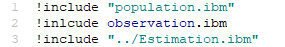
\includegraphics[scale=1]{Figures/config.png}
	\caption{\textbf{Example of using the \config\ command !\texttt{\emph{include}}
			\texttt{\emph{file}} .}}\label{fig:config_file_1}
\end{figure}

\subsection{\I{Redirecting standard output}\label{sec:redirecting-stdout}}

\IBM\ uses the \texttt{standard output}\index{standard output} stream to display run-time information. The \I{standard error} stream is used by \IBM\ to output the program exit status and run-time errors. We suggest redirecting both the standard output and standard error into files\index{Redirecting standard out}\index{Redirecting standard error}. With the bash shell (on Linux systems), you can do this using the command structure,

\begin{verbatim} (ibm [arguments] > out) >& err &\end{verbatim}

It may be useful to redirect the standard input, especially if you're using \IBM\ inside a batch job software, i.e. 

\begin{verbatim} (ibm [arguments] > out < /dev/null) >& err &\end{verbatim}

On Microsoft Windows systems, you can redirect to standard output using,

\begin{verbatim} ibm [arguments] > out\end{verbatim}

And, on some Microsoft Windows systems (e.g., Windows10), you can redirect to both standard output and standard error, using the syntax, 

\begin{verbatim} ibm [arguments] > out 2> err\end{verbatim}

Note that \IBM\ outputs a few lines of header information to the output (e.g. Figure~\ref{fig:log_file_1}). The header\index{Output header information} consists of the program name and version, the arguments passed to \IBM\ from the command line, the date and time that the program was called (derived from the system time), the user name, and the machine name (including the operating system and the process identification number). These can be used to track outputs as well as identifying the version of \IBM\ used to run the model.


\subsection{\I{Command line arguments}\label{sec:command-line-arguments}}

The call to \IBM\ is of the following form: 

\texttt{\ibm [-c \emph{config\_file}] [\emph{task}] [\emph{options}]}

where, 

\begin{description}
  \item [\texttt{-c \emph{config\_file}}] Define the \config\ for \IBM\ (if omitted, \IBM\ looks for a file named \texttt{config.ibm})
\end{description}

and where \emph{task} must be one of the following (\textbf{[]} indicates a secondary label to call the task, e.g. \textbf{\texttt{-h}} will execute the same task as \textbf{\texttt{--help}}),

\begin{description}
\item [\texttt{-h [--help]}] Display help (this page)
\item [\texttt{-l [--licence]}] Display the reference for the software license (GPL v2)
\item [\texttt{-v [--version]}] Display the \IBM\ version number

\item [\texttt{-r [--run]}] \emph{Run} the model once using the parameter values in the \config, or optionally, with the values from the file denoted with the command line argument \texttt{-i \emph{file}}

\end{description}

and where the following optional arguments\index{Optional command line arguments} [\emph{options}] may be specified,

\begin{description}
\item [\texttt{-g [--seed]\emph{seed}}]  \emph{Seed} the random number \emph{generator} with \texttt{\emph{seed}}, a positive (long) integer value (note, if \texttt{-g} is not specified, then \IBM\ will  generate a random number seed based on the computer clock time)

\item [\texttt{--loglevel}] arg = \{trace, finest, fine, medium\} (see Section \ref{sec:report-section})
\end{description}

\subsection{Constructing the \IBM\ \config s \label{constructing-config}}\index{Input configuration file syntax}

The model definition, parameters, observations, and reports are specified in \config s:
 
\begin{description}

\item Population input (Section \ref{sec:population-section}) specifies the model structure, population dynamics, and other associated parameters;
\item Observation input (Section \ref{sec:observation-section}) contains all the observations data available to the model and  describes how the observed values should be formatted, how \IBM\ calculates the expected values, and the likelihoods available for each type of observation; and
\item Report input (Section \ref{sec:report-section}) specifies any output required.
\end{description}

The command and subcommand syntax to be used in each of these configuration files are listed in Sections \ref{sec:population-syntax} (Population), \ref{sec:observation-syntax} (Observation) and \ref{sec:report-syntax} (Report).

\subsubsection{Commands}\index{Commands}

\IBM\ has a range of commands that define the model structure, processes, observations, and how tasks are carried out. There are three types of commands, 

\begin{enumerate}
\item Commands that have an argument and do not have subcommands (for example, !\texttt{\emph{include}}\ \argument{\emph{file}})
\item Commands that have a label and subcommands (for example \command{process} must have a label, and has subcommands)
\item Commands that do not have either a label or argument, but have subcommands (for example \command{model})
\end{enumerate}

Commands that have a label must have a unique label, i.e., the label cannot be used on more than one command of that type. The labels can contain alpha numeric characters, period (`.'), underscore (`\_') and dash (`-'). Labels must not contain white-space, or other characters that are not letters, numbers, dash, period or an underscore. For example,

{\small{\begin{verbatim}
@process NaturalMortality
or
!include MyModelSpecification.csl2
		\end{verbatim}}}

\subsubsection{Subcommands}\index{Commands ! Subcommands}

\IBM\ subcommands are used for defining options and parameter values related to a particular command. Subcommands always take an argument which is one of a specific \emph{type}. The argument \emph{types} acceptable for each subcommand are defined in Section \ref{sec:syntax}, and are summarised below. 

Like commands (\command{command}), subcommands and their arguments are not order specific --- except that that all subcommands of a given command must appear before the next \command{command} block. \IBM\ may report an error if they are not supplied in this way. However, in some circumstances a different order may result in a valid, but unintended set of actions, leading to possible errors in your expected results.  

The argument type for a subcommand can be either\index{Subcommand argument type}:

\begin{tabular}{ll}
\textbf{switch} & true/false\\ 
\textbf{integer}& an integer number,\\
\textbf{integer vector} & a vector of integer numbers,\\
\textbf{integer range} & a range of integer numbers separated by a colon, e.g. 1994:1996 is \\ & expanded to an integer vector of values (1994 1995 1996),\\
\textbf{constant} & a real number (i.e. double),\\
\textbf{real vector} & a vector of real numbers (i.e. vector of doubles),\\
\textbf{real} & a real number that can be estimated (i.e. float),\\
\textbf{addressable} & a real number that can be referenced but not estimated (i.e. addressable double),\\
\textbf{addressable vector} & a vector of real numbers that can be referenced but not estimated (i.e. vector of addressable \\ & doubles),\\
\textbf{string} & a categorical (string) value, or\\
\textbf{string vector} & a vector of categorical values.
\end{tabular}

Switches are parameters which are either true or false. Enter \emph{true} as \argument{true} or \argument{t}, and \emph{false} as \argument{false} or \argument{f}. 

Integers must be entered as integers (i.e., if \subcommand{year}\ is an integer then use 2008, not 2008.0)

Arguments of type integer vector, integer range, constant vector, real vector, addressable vector, or categorical vector must contain one or more entries on a row, separated by white space (tabs or spaces). 

Note that parameters defined as addressable with the subcommand type \texttt{addressable} or \texttt{addressable vector} are usually derived IBM and are not directly estimable. As such, they can be acted upon by the model (e.g. called by various processes; have priors and/or penalties assigned to them), but they do not directly contribute to any estimation within the model

\subsubsection{The command-block format}\index{Command block format}
Each command-block consists of a single command (starting with the symbol \command{}) and, for most commands, a unique label or an argument. Each command is then followed by its subcommands and their arguments, e.g., 

\begin{multicols}{3}
	\begin{description}
		\item \command{command}, or
		\item \subcommand{subcommand} \subcommand{argument}
		\item \subcommand{subcommand} \subcommand{argument}
		\item .
		\item .
		\item etc.
		\item \command{command} \subcommand{argument}, or
		\item \subcommand{subcommand} \subcommand{argument}
		\item \subcommand{subcommand} \subcommand{argument}
		\item .
		\item .
		\item etc.
		\item \command{command} \subcommand{\emph{label}}
		\item \subcommand{subcommand} \subcommand{argument}
		\item \subcommand{subcommand} \subcommand{argument}
		\item .
		\item .
		\item etc.
		\end{description}
	\end{multicols}


Blank lines are ignored, as is extra white space (i.e., tabs and spaces) between arguments. However, to start command block the \command{} character must be the first character on the line and must not be preceded by any white space. Each input file must end with a carriage return.

There is no need to mark the end of a command block. This is automatically recognized by either the end of the file, section, or the start of the next command block (which is marked by the \command{} on the first character of a line). Note, however, that the !\texttt{\emph{include}} is the only exception to this rule (see Section \ref{sec:general-syntax}\index{Command ! Include files} for details of the use of !\texttt{\emph{include}}). 

Commands, sub-commands and arguments in the \config s are not case sensitive. Labels and variable values are case sensitive. Also, on a Linux system, external calls to files are case sensitive (i.e., when using !\texttt{\emph{include}} \subcommand{\emph{file}}, the argument \subcommand{\emph{file}} will be case sensitive). 


\subsubsection{\I{Commenting out lines}}\index{Comments}
Text on a line that follows an \commentline\ is considered to be a comment and is ignored. To comment out a group of commands or subcommands, use a \commentline\ at the beginning of each line to be ignored.

Alternatively, to comment out an entire block or section place a \commentstart\ as the first character on the line to start the comment block, then end it with \commentend. All lines (including line breaks) between \commentstart\ and \commentend\ inclusive are ignored. 
{\small{\begin{verbatim}
		# This is a comment and will be ignored
		@process NaturalMortality
		m 0.2
		/* 
		This block of code 
		is a comment and
		will be ignored
		*/
		\end{verbatim}}}

\subsubsection{Determining \IBM\ parameter names\label{sec:parameter-names}\index{Determining parameter names}\index{Parameter names}}

When \IBM\ processes an \config\ it translates each command block and each subcommand block into a unique \IBM\ object, each with a unique parameter name. For commands, this parameter name is simply the command label. For subcommands, the parameter name format is either: 

\begin{description}
\item \texttt{command[label].subcommand} if the command has a label, or
\item \texttt{command.subcommand} if the command has no label, or
\item \texttt{command[label].subcommand\{i\}} if the command has a label and the subcommand arguments are a vector, and we are accessing the  \emph{i}th element of that vector. 
\item \texttt{command[label].subcommand\{i:j\}} if the command has a label, and the subcommand arguments are a vector, and we are accessing the elements from $i$ to $j$ (inclusive) of that vector.
\end{description} 

The unique parameter name is used to reference that unique parameter when, for example, estimating, applying a penalty, projecting, time varying or applying a profile. For example, the parameter name of the Natural mortality rates subcommand \subcommand{m} of the command \command{process} with the label \argument{NaturalMortality} is category related and so, the syntax to reference all m related categories is, 

\texttt{process[NaturalMortality].m}

Or, the syntax to specify a single category for which to apply the natural mortality process is,

\texttt{process[NaturalMortality].m\{male\}}

All labels (parameter names) are user specified. As such, naming conventions are non-restrictive and can be model specific.

\subsection{\IBM\ exit status values\index{Exit status value}}
Whether \IBM\ completes its task successfully or errors out gracefully, it returns a single exit status value 'completed' to the standard output. Error messages will be printed to the console. When configuration errors are found \IBM\ will print error messages, along with the associated files and line numbers where the errors were identified, for example,

{\small{\begin{verbatim}
	#1: At line 15 in Reports.ibm: Parameter '{' is not supported
\end{verbatim}}}	

\clearemptydoublepage{}
\section{\I{The population section}\label{sec:population-section}}

\subsection{Introduction}
The population section\index{Population section} specifies the model of the population dynamics. It describes the model structure (population structure), defines the population processes (e.g., recruitment, migration, and mortality), the selectivities, and associated parameters.

The population section consists of several components, including:
\begin{itemize}
  \item The population structure;
  \item Model initialisation (i.e., the state of the partition at the start of the first year)\index{Initialisation}\index{Model ! initialisation};
  \item The years over which the model runs (i.e., the start and end years of the model)
  \item The annual cycle (time-steps and processes that are applied in each time-step)\index{Annual cycle};
  \item The specification and parameters of the population processes (i.e., processes that add, remove individuals to or from the partition, or shift numbers between ages and categories in the partition);
  \item Selectivities;
  \item Parameter values and their definitions; and
  \item Derived IBM, required as parameters for some processes (e.g. mature biomass to resolve any density dependent processes, such as the spawner-recruit relationship in a recruitment process).
\end{itemize}

\subsection{\I{Population structure}}\label{sub:sec:pop_sec}
The basic structure of the population section of a \IBM\ model is defined in terms of an annual cycle, time steps, states, and transitions.

The annual cycle defines what processes happen in each model year, and in what sequence. \IBM\ runs on an annual cycle rather than, for example, a 6-monthly cycle.

Each year is split into one or more time steps, with at least one process occurring in each time step. Each time step can be thought of as representing a particular part of the calendar year, or time steps can be treated as an abstract sequence of events. In every time step, there exists a mortality block: a group of consecutive mortality-based processes, where individuals are removed from the partition (see Section~\ref{sec:mortality_block}).

The state is the current status of the population at any given time. The state can change one or more times in each time step of every year. The state object must contain sufficient information to figure out how the underlying population changes over time (given a model and a complete set of parameters).

The state can undergo a number of possible changes, called transitions. Transitions are accomplished by processes, including: recruitment, natural mortality, anthropogenic mortality, ageing, migration, tagging events, and maturation. 

The division of the year into an arbitrary number of time steps allows the user to specify the exact order in which processes and observations occur throughout the year. The user needs to specify the time step in which each process occurs. If more than one process occurs in the same time step, the order in which to apply each process is specified in the \command{time\_step} block.

The key element of the state is the spatial world view, which holds all the entities.

An example, to specify a model with 2 categories (male and female) with ages 1-20 (with the last age a plus group) and an age-length relationship defined with the label \texttt{male\_growth} and \texttt{female\_growth}, then the \texttt{@model} block is specified as:
{\small{\begin{verbatim}
		@model
		start_year
		final_year
		min_age 1
		max_age 20
		age_plus_group True
		initialisation_phases iphase
		time_steps step1 step2 step 3
\end{verbatim}}}

\subsection{\I{The state object and the partition}}



\subsection{\I{Time sequences}}

The time sequence of the model is defined in the following parts;
\begin{itemize}
  \item \I{Annual cycle}
  \item \I{Mortality blocks}
  \item \I{Initialisation}
  \item \I{Model run years}
  \item \I{Projection year}s
\end{itemize}

\subsubsection{\I{Annual cycle}}
The annual cycle is implemented as a set of processes that occur, in a user-defined order, within each year. Time-steps are used to break the annual cycle into separate components, and allow observations to be associated with different time periods and processes. Any number of processes can occur within each time-step, in any order (although there are limitations around mortality based processes - see Section~\ref{sec:mortality_block}) and can occur multiple times within each time-step. Note that time-steps are not implemented during the initialisation phases (effectively, there is only one time-step), and that the annual cycle in the initialisation phases can, optionally, be different from that which is applied during the model years.

\subsubsection{\I{Mortality blocks}}\label{sec:mortality_block}

For every time step in an annual cycle there is an associated \emph{mortality block}. Mortality blocks are a key concept in \IBM.

Mortality blocks are used to define the `point' in the model time sequence when observations (see Section~\ref{sec:observation-section}) are evaluated, and derived IBM (see Section~\ref{sec:derived-IBM}) are calculated.

A mortality block is defined as a consecutive sequence of mortality processes within a time step. The processes that are mortality processes are all pre-defined in \IBM, and cannot be modified. These mortality processes are described in subsection~\ref{sec:mortality}. 

\IBM\ requires that each time step has exactly one mortality block. To achieve this, either all the mortality processes in a time step must be sequential (i.e., there can not be a non-mortality process between any two mortality processes within any one time step); or if no mortality processes occur in a time step then the mortality block is defined to occur at the end of the time step. 

\IBM\ will error out if more than one mortality block occurs in a single time step. 


\subsubsection{\I{Initialisation}}\label{subsec:initialisation}
Initialisation is the process of determining the world's state just before \subcommand{start\_year}, whether it be equilibrium/steady state or some other initial state for the model (e.g exploited), prior to the start year of the model. This can be computationally expensive if a plus group is present in the partition.

Currently users can only initialise the partition via an iterative process. \IBM\ does a few tricks to help speed up the initialisation. The first thing \IBM\ does is gets the parameter \subcommand{number\_of\_agents} and spits that number of agents uniformly, over the spatial domain, alternatively the user could supply a layer \subcommand{layer\_label} of proportions to seed the initial spatial distribution. This layer should sum to one so that the model initially seeds \subcommand{number\_of\_agents}. When the \IBM\ seeds the initial number of agents it also randomly assigns the agents an age based on an exponential distribution where the parameter $\lambda$ of the exponential distribution is set by the command on the \command{model}, \subcommand{initialisation\_z\_seed}. We suggest setting this command to the assumed natural mortality of the model. To see what age structure this would look like you can quickly use \R\ to visualise. by running the following code in an \R\ terminal you could see.

\begin{lstlisting}
Z_param = 0.2;
agents_per_cell = 1000;
hist(rexp(agents_per_cell,Z_param), breaks = 30, xlab = "age", ylab = "frequency", main = "Initial age structure in each cell")
\end{lstlisting}

Once \IBM\ has seeded the agents, it iterates over the annual cycle to change an approximated initialisation state to one that is more like what would occur for your annual cycle, this is controlled by the \subcommand{years} command in the \command{initialisation} block. The number of iterations in the iterative initialisation can effect the model output, and these should be chosen to be large enough to allow the population state to fully converge. We recommend that a period of about two generations to ensure convergence. \IBM\ can be requested to report a number of convergence statistics that can assist the user in determining the level of convergence.

In addition, the iterative initialisation phase can optionally be stopped early if some user defined convergence criteria is met. For a list of supplied years in the initialisation phase, convergence is defined as met if the proportional absolute summed difference between the state in year $t-1$ and the state in year $t$ ($\widehat{\lambda}$) is less than a user defined $\lambda$ where, 
\begin{equation}
  \widehat{\lambda} = \frac{\sum\limits_{i} \sum\limits_{j} \left|\text{element}(i,j)_t - \text{element}(i,j)_{t-1} \right|}{\sum\limits_{i} \sum\limits_{j} \frac{}{}\text{element}(i,j)_t}
\end{equation}

Hence, for an iterative initialisation you need to define:
\begin{itemize}
  \item The initialisation phases,
  \item The number of years in each phase, and
  \item the natural mortality process
  \item the growth process
\end{itemize}

Because the initialisation phase is responsible for seeding the initial agents, users must specify processes that the initialisation phase can seed parameters to agents. To see how parameters are set for each individual agent, users should see the individual processes in this Section~\ref{sec:process}.

An example of the syntax to implement this would be,
{\small{\begin{verbatim}
@model
...
initialisation_phases Iterative_initialisation

@initialisation_phase Iterative_initialisation
type iterative
years 50
lambda 0.0001
convergence_years 20 40
layer_label Base
growth_process_label von_bert
natural_mortality_process_label natural_mort
\end{verbatim}}}

\subsection{\I{Population processes}}\label{sec:process}

\subsubsection{\I{Ageing}}
Ageing is an implicit process in the model, Each agent that is created or recruited gets assigned an birth year. This means that when ever we want to ask for the agent we just calculate \subcommand{current\_year - birth\_year}, thus there is no explicit ageing process. Note that we do return the \subcommand{max\_age} of the model, if the agent is older than that age (so we only work with the truncated age distribution).


This means every fish automatically ages by one at the end of the year, or you could think of ageing a fish at the very beginning of the year (tomayto, tomahto), just be aware that you don't  have control over that, but if you want to account for growth in between annual increments that is possible via time step proportion increments, see growth processes for more information.

\subsubsection{\I{Recruitment}}

\paragraph{\I{Constant recruitment}}\label{subsubsec:constant-recruitment}

\subsubsection{\I{Mortality}\label{sec:mortality}}

\paragraph{Constant mortality rate}

\subsection{\I{Derived Quantities}\label{sec:derived-IBM}}

\subsection{\I{Growth}\label{sec:age-at-age}}

\subsection{\I{Length-weight relationship}\label{sec:mean-weight}}
Growth currently means updating length and weight for an agent, if the Von Bertalanffy formula currently is used (currently the default in agent class for initialising length) it follows the following formula

\begin{equation}\label{VB}
	\Delta L = (L_{\infty} - L)(1 - e^k)
\end{equation}


If the basic length weight formulation is used, then an agents weight follows the following formula

\begin{equation}\label{mean_weight}
\bar{w} = aL^b
\end{equation}

Scaling the model agents up to the population biomass estimates is done via a stock specific scalar.}

\subsection{\I{Selectivities}\label{sec:selectivities}}
A selectivity is a function that can have a different value for each age class. Selectivities are used throughout \IBM\ to interpret observations (Section \ref{sec:estimation-section}) or to modify the effects of processes on each age class (Section \ref{sec:population-section}). \IBM\ implements a number of different parametric forms, including logistic, knife edge, and double normal selectivities. Selectivities are defined in there own command block (\command{selectivity}), where the unique label is used by observations or processes to identify which selectivity to apply.

Selectivities are indexed by age, with indices from \argument{min\_age} to \argument{max\_age}. For example, for a logistic age-based selectivity with $50\%$ selected at age $5$ and $95\%$ selected at age $7$, would be defined by the \subcommand{type}=\argument{logistic} with parameters $a_{50}=5$ and $a_{to95}=(7-5)=2$. The value of the selectivity at age $x=7$ is $0.95$, and the value at age $x=3$ is $0.05$. Note, while selectivities can be length based, use with caution as more testing is needed for this functionality.

The function values for some choices of parameters, for some selectivities, can result in a computer numeric overflow error (i.e., the number calculated from parameter values is either too large or too small to be represented in computer memory). \IBM\ implements range checks on some parameters to test for a possible numeric overflow error before attempting to calculate function values. For example, the logistic selectivity is implemented such that if $(a_{50}-x)/a_{to95} > 5$ then the value of the selectivity at $x=0$, i.e., for $a_{50}=5$, $a_{to95}=0.1$, then the value of the selectivity at $x=1$, without range checking would be $7.1 \times 10^{-52}$. With range checking, that value is $0$ (as $(a_{50}-x)/a_{to95}=40 > 5$).

The available selectivities are;

\begin{itemize}
  \item Constant
  \item Knife-edge
  \item All values
  \item All values bounded
  \item Increasing
  \item Logistic
  \item Inverse logistic
  \item Logistic producing
  \item Double normal
  \item Double exponential
% \item Cubic spline (Not yet implemented)
\end{itemize}

The available selectivities are described below.

\subsubsection[Constant]{{constant}}

\begin{equation}
f(x)=C
\end{equation}

The constant selectivity has the estimable parameter C. 

\subsubsection[Knife-edge]{\argument{knife\_edge}}
\begin{equation}
f(x)= \begin{cases}
  0, & \text{if $x < E$} \\
  \alpha, & \text{if $x \ge E$}\\ 
  \end{cases} 
\end{equation}

The knife-edge ogive has the estimable parameter E and a scaling parameter $\alpha$, where the default value of $\alpha = 1$.

\subsubsection[All-values]{\argument{all\_values}}\index{Selectivities!All-values}

\begin{equation}
f(x)=V_x
\end{equation}

The all-values selectivity has estimable parameters $V_{low}$, $V_{low+1}$ \ldots $V_{high}$. Here, you need to provide the selectivity value for each age class.

\subsubsection[All-values-bounded]{\argument{all\_values\_bounded}}\index{Selectivities!All-values-bounded}

\begin{equation}
f(x)=\begin{cases}
		 0, & \text{if $x < L$} \\
		 V_x, & \text{if $L \le x \le H$} \\
		 V_H, & \text{if $x > H$}
  \end{cases}
\end{equation}

The all-values-bounded selectivity has non-estimable parameters L and H. The estimable parameters are $V_L$, $V_{L+1}$ \ldots $V_H$. Here, you need to provide an selectivity value for each age class from $L \ldots H$.

\subsubsection[Increasing]{\argument{increasing}}\index{Selectivities!Increasing}

\begin{equation} 
f(x)=\begin{cases}
	  0, & \text{if $x < L$} \\
	  f(x-1)+ \pi_x(\alpha-f(x-1)), & \text{if $L \le x \le H$} \\
	  f(\alpha), & \text{if $x \ge H$} \\  
  \end{cases}
\end{equation}

The increasing ogive has non-estimable parameters $L$ and $H$. The estimable parameters are $\pi_L$, $\pi_{L+1}$ \ldots $\pi_H$ (but if these are estimated, they should always be constrained to be between 0 and 1). $\alpha$ is a scaling parameter, with default value of $\alpha = 1$. Note that the increasing ogive is similar to the all-values-bounded ogive, but is constrained to be non-decreasing.

\subsubsection[Logistic]{\argument{logistic}}\index{Selectivities!Logistic}

\begin{equation}
  f(x) = \alpha / [1+19^{(a_{50}-x)/a_{to95}}]
\end{equation}
 
The logistic selectivity has estimable parameters $a_{50}$ and $a_{to95}$. $\alpha$ is a scaling parameter, with default value of $\alpha = 1$. The logistic selectivity takes values $0.5 \alpha$ at $x=a_{50}$ and $0.95 \alpha$ at $x=a_{50}+a_{to95}$. 

\subsubsection[Inverse logistic]{\argument{inverse\_logistic}}\index{Selectivities!Inverse-logistic}

\begin{equation}
  f(x) = \alpha - \alpha / [1+19^{(a_{50}-x)/a_{to95}}]
\end{equation}
 
The inverse logistic selectivity has estimable parameters $a_{50}$ and $a_{to95}$. $\alpha$ is a scaling parameter, with default value of $\alpha = 1$. The logistic selectivity takes values $0.5 \alpha$ at $x=a_{50}$ and $0.95 \alpha$ at $x=a_{50}-a_{to95}$. 

\subsubsection[Logistic producing]{\argument{logistic\_producing}}\index{Selectivities!Logistic-producing}

\begin{equation} 
f(x)=\begin{cases}
	  0, & \text{if $x < L$} \\
	  \lambda(L), & \text{if $x=L$} \\
	  \left( \lambda(x)-\lambda(x-1) \right) / \left( 1-\lambda(x-1) \right), & \text{if $L < x < H$} \\
	  1, & \text{if $x \ge H$} \\  
  \end{cases}
\end{equation}

The logistic-producing selectivity has the non-estimable parameters $L$ and $H$, and has estimable parameters $a_{50}$ and $a_{to95}$. $\alpha$ is a scaling parameter, with default value of $\alpha = 1$. For category transitions, $f(x)$ represents the proportion moving, not the proportion that have moved. This selectivity was designed for use in an age-based model to model maturity. In such a model, a logistic-producing maturation selectivity will (in the absence of other influences) make the proportions mature follow a logistic curve with parameters $a_{50}$, $a_{to95}$.

\subsubsection[Double-normal]{\argument{double\_normal}}\index{Selectivities!Double-normal}

\begin{equation}
  f(x) = \begin{cases}
    \alpha 2^{-[(x- \mu)/\sigma_L ]^2}, & \text{if $x \leq \mu$} \\
    \alpha 2^{-[(x- \mu)/\sigma_R ]^2}, & \text{if $x \ge \mu$}\\
  \end{cases}
\end{equation} 

The double-normal selectivity has estimable parameters $a_1$, $s_L$, and $s_R$. $\alpha$ is a scaling parameter, with default value of $\alpha = 1$. It has values $\alpha$ at $x=a_1$, and $0.5 \alpha$ at $x=a_1-s_L$ and $x=a_1+s_R$. 

\subsubsection[Double-exponential]{\argument{double\_exponential}}\index{Selectivities!Double-exponential}

\begin{equation} 
f(x)=\begin{cases}
	  \alpha y_0(y_1 / y_0)^{(x-x_0)/(x_1-x_0)}, & \text{if $x \le x_0$} \\
	  \alpha y_0(y_2 / y_0)^{(x-x_0)/(x_2-x_0)}, & \text{if $x > x_0$} \\
  \end{cases}
\end{equation}

The double-exponential selectivity has non-estimable parameters $x_1$ and $x_2$, and estimable parameters $x_0$, $y_0$, $y_1$, and $y_2$.  $\alpha$ is a scaling parameter, with default value of $\alpha = 1$. It can be `U-shaped'. Bounds for $x_0$ must be such that $x_1 < x_0 < x_2$. With $\alpha=1$, the selectivity passes through the points $(x_1, y)$, $(x_0, y_0)$, and $(x_2, y_2)$. If both $y_1$ and $y_2$ are greater than $y_0$ the selectivity is `U-shaped' with minimum at $(x_0, y_0)$.

%\subsubsection[Spline]{\argument{spline}}\index{Selectivities!Spline}
%
%The spline selectivity implements a cubic spline that has non-estimable knots, and an estimable value for each knot. The cubic spline is either (i) a natural splines where the second derivatives are set to 0 at the boundaries, i.e., the values at the boundaries are horizontal, (ii) a spline with a fixed first derivative at the boundaries (linear, but not necessarily horizontal) and (iii) spline which turns into a parabola at the boundaries. 
%


Selectivities \subcommand{all\_values} and \subcommand{all\_values\_bounded} can be addressed in additional priors using the following syntax,

{\small{\begin{verbatim}
		@selectivity maturity
		type all_values
		v 0.001 0.1 0.2 0.3 0.4 0.3 0.2 0.1
		
		## encourage ages 3-8 to be smooth.
		@additional_prior smooth_maturity
		type vector_smooth
		parameter selectivity[maturity].values{3:8}
		
		\end{verbatim}}}


\clearemptydoublepage{}
\section{\I{The estimation section}\label{sec:estimation-section}}
\subsection{\I{The numerical differences minimiser}}\label{subsec:num_diff}

The minimiser has three kinds of (non-error) exit status, depending on the minimiser: 

\begin{enumerate}
\item Successful convergence (suggests you have found a local minimum, at least).
\item Convergence failure (you have not reached a local minimum, though you may deem yourself to be `close enough' at your own risk).
\item Convergence unclear (the minimiser halted but was unable to determine if convergence occurred. You may be at a local minimum, although you should check by restarting the minimiser at the final values of the estimated parameters).
\end{enumerate}

You can choose the maximum number of quasi-Newton iterations\index{Quasi-Newton iterations} and objective function evaluations\index{Objective function evaluations} allotted to the minimiser. If it exceeds either limit, it exits with a convergence failure\index{Convergence failure}. We recommend large numbers of evaluations and iterations (at least the defaults of 300 and 1000) unless you successfully reach convergence with less. 

We want to stress that the minimisers are local optimisation algorithms trying to solve a global optimisation problem. What this means is that, even if you get a 'successful convergence'\index{Successful convergence} message, your solution may be only a local minimum\index{Local minimums}, not a global one. To diagnose this problem, try doing multiple runs from different starting points and comparing the results, or doing profiles of one or more key parameters and seeing if any of the profiled estimates finds a better optimum than than the original point estimate.


{\small{\begin{verbatim}
@minimiser numerical_diff
type numerical_differences
tolerance 1e-6
iterations 2500
evaluations 4000
\end{verbatim}}}

\clearemptydoublepage{}
\section{The observation section\label{sec:observation-section}}
This section describes the observations that \IBM\ can generate during run time. \IBM\ calculates expectations of all the agents that are user defined, and then adds observation error via simulating through a distribution with a user defined observation error value.
\subsection{\I{Observations}\label{sec:Observations}\index{Observations}}

\subsubsection{Process Removals By Age}\label{subsubsec:catch_at_age}\index{Observations!Process Removals By Age}
This observation class aggregates age frequency over a user defined spatial area from a \subcommand{mortality\_event\_biomass} and \subcommand{mortality\_baranov} process. This class can add ageing error onto the expectation, to account for ageing error which is a source of uncertainty in ageing fish. An example of how you would set this observation up and show some of the flexibilities in the spatial resolution see the syntax below for a 6 area model.

{\small{\begin{verbatim}
@process fishing
type mortality_event_biomass
years 2000
catch_layers catch_2000
selectivity fishing_selectivity

@layer catch_2000
type numeric
table_layer
600 500 400
1034 601 200
903 450 100
end_table

@layer cells
type categorical
table_layer
r1-c1 r1-c2 r1-c3
r2-c1 r2-c2 r2-c3
r3-c1 r3-c2 r3-c3
end_table

@observation fishery_age
type process_removals_by_age
cell_layer cells
cells r1-c1 r1-c2 r1-c3 r2-c1 r2-c2 r2-c3 r3-c1 r3-c2 r3-c3
simulation_likelihood multinomial
process_label fishing
years 2000
min_age 0
max_age 28
plus_group true
table error_values
2000 10000
end_table
\end{verbatim}}}

The above syntax asks for an age frequency for each cell in the spatial domain through the link to the categorical layer. You could easily summarise the age frequency over the whole spatial domain by changing the categorical layer as shown below

{\small{\begin{verbatim}
@layer cells
type categorical
table_layer
single_cell single_cell single_cell
single_cell single_cell single_cell
single_cell single_cell single_cell
end_table

@observation fishery_age
type process_removals_by_age
cell_layer cells
cells single_cell
simulation_likelihood multinomial
process_label fishing
years 2000
min_age 0
max_age 28
plus_group true
table error_values
2000 10000
end_table
\end{verbatim}}}

Hopefully the above example illustrates how much control the user has in specifying what information they want to extract.

\subsubsection{Biomass}\label{subsubsec:biomass}\index{Observations!Biomass}
This observation summarises the biomass over a selected number of agents in a time step over the mortality block (Section~\ref{sec:mortality_block}), for user defined spatial areas. \IBM\ does an interpolation similar to the derived quantities if the user wishes to extract a biomass observation that represents a proportion of mortality being taken.

{\small{\begin{verbatim}
@observation survey_index
type biomass
years 1990:2013
time_step Summer
catchability 0.342
proportion_through_mortality_block 1.0 ## take snapshot at the end of timestep
simulation_likelihood lognormal
error_value 0.2 * 24
selectivities Sel_survey
cell_layer cells
cells r1-c1 r2-c1 r3-c1 
\end{verbatim}}}

\subsubsection{Proportions at age}\label{subsubsec:Proportions_at_age}\index{Observations!Proportions at age}
This observation summarises the proportions at age for selected number of agents in a time step over the mortality block (Section~\ref{sec:mortality_block})

{\small{\begin{verbatim}
@observation survey_age_comp
type proportions_at_age
simulation_likelihood multinomial
years 1990:1995
min_age 0
max_age 20
plus_group true
ageing_error none
table error_values
1990 300
1991 300
1992 300
1993 300
1994 300
1995 300
end_table
cell_layer cells
cells r1-c1 r2-c1 r3-c1
\end{verbatim}}}


\subsubsection{Age frequency from scaled length frequency}\label{subsubsec:Mortalitysubsamle}\index{Observations!Age frequency from scaled length frequency}
This observation class, generates an age frequency by getting all agents removed by an F method in user defined stratum, and returns a sub-sample of age and lengths that is used to generate an age length key. The user can ask for ageing-error to be applied to when generating an age length key, using the  \command{ageing\_error} block (see Section~\ref{subsec:ageing_error}). Calculations currently follow the following algorithm for each spatial stratum,

\begin{enumerate}
	\item randomly sub sample fishery to calculate length frequency
	\item within the sampled fish for length frequency, sub sample ages based on the \subcommand{age\_allocation\_method} command
	\item apply ageing error to the ages.
\end{enumerate}

\begin{equation}
N_{n,a} = \sum_l K_{a,l,n} N_{l,n}
\end{equation}

where $K_{a,l,n}$ is the age length key for stratum $n$, $N_{l,n}$ is the numbers at length which can be a sub sample of the fishery, this is controlled by the input table \subcommand{proportion\_lf\_sampled}. There are three methods for allocating ages for a single age length key, these are \subcommand{random}, \subcommand{equal}, \subcommand{proportional}. Random will uniformly sample without replacement, Equal will put equal amount of ages in each length bin that is non-zero, and proportional will distribute the number of ages, proportional to the length frequency.

\begin{equation}
N_{a} = \sum_n \sum_s N_{n,a,s}
\end{equation}

At some point when I return to this I wont to add sex if sexual dimorphism is evident among agents, see below for more improvements that I will be adding to this class.

{\small{\begin{verbatim}
@observation scaled_age_freq
type mortality_scaled_age_frequency
years 1991
process_label summer_fishery
ageing_error none
stratum_weighting_method biomass
layer_of_stratum_definitions summery_fishery_catch_at_age_stratum
stratums_to_include Inshore Offshore
age_allocation_method proportional

table samples ## number of individuals randomly selected to calculate age-length key
year   Inshore    Offshore
1991   400        200
end_table

table proportion_lf_sampled ## proportion of catch that is sampled for Length frequency
year   Inshore    Offshore
1991   0.8        0.7
end_table
simulation_likelihood multinomial

@layer summery_fishery_catch_at_age_stratum
type categorical
table layer 
Inshore Inshore Offshore Offshore Offshore
Inshore Inshore Offshore Offshore Offshore
Inshore Inshore Offshore Offshore Offshore
Inshore Inshore Offshore Offshore Offshore
end_table
\end{verbatim}}}


\subsubsection{Age frequency from scaled length frequency for Mortality Event Biomass process}\label{subsubsec:MortalityEventBiomasssubsamle}\index{Observations!Age frequency from Mortality Event Biomass}
This observation class, is an extension of the class Age frequency from scaled length frequency (Section~\ref{subsubsec:Mortalitysubsamle}) and is the recommended age-length method when generating mortality based age-frequencies from process of type \subcommand{mortality\_event\_biomass}. This is mainly because the process \subcommand{mortality\_event\_biomass} allows for multiple fisheries (gear types/vulnerabilities) and so generally we want to generate an age-frequency for a specific fishery. The algorithm is similar to that of the class is derives from with the following steps run.

For each Stratum identify all agents that are measured for Length frequency.
\begin{enumerate}
	\item randomly sub sample cells that are within each stratum (can have many) 
	\item For each cell randomly select all available agents for measuring length frequency (denoted by table \subcommand{proportion\_lf\_sampled})
\end{enumerate}
For all agents measured for length within the stratum ($N_n$) sub-sample agents available for otolith reading with a length based probability according to the subcommand \subcommand{age\_allocation\_method}. Where the probabilities are defined for an agent of length $l$ as,
\begin{enumerate}
		\item \subcommand{random} $\frac{1}{N_n}$
		\item \subcommand{proportional} $\frac{N_{l,n}}{N_n}$
		\item \subcommand{equal} $\frac{1}{n_l}$
\end{enumerate}
where $N_{l,n}$ is the numbers measured for length in length bin $l$ in stratum $n$ and $n_l$ is the number of length bins that are non zero. When sub-sampling for age occurs this sampling is \textbf{without} replacement. The algorithm will do it's best to allocate ages according to these probabilities, if after so many attempts it can't fully allocate the number of otoliths according to these probabilities. It will abandon random methods and try systematically find fish to complete the distribution. This will occur when is a low probability that by its very definition will take a long time to randomly generate a sample of. Once we have randomly sub-sampled ages we calculate an Age Length Key (ALK) (represented as proportions) and calculate final ages following. Ageing error is applied in the age-length key, so if an agent is of age 3 but misclassified as age 4 then it is put in the ALK as age 4.

\begin{equation}
N_{n,a} = \sum_l K_{a,l,n} N_{l,n}
\end{equation}

\begin{equation}
N_{a} = \sum_n \sum_s N_{n,a,s}
\end{equation}


{\small{\begin{verbatim}
		@observation scaled_age_freq
		type mortality_event_biomass_scaled_age_frequency
		years 1991
		process_label summer_fishery
		fishery_label fisheryTrwl
		ageing_error none
		stratum_weighting_method biomass
		layer_of_stratum_definitions summery_fishery_catch_at_age_stratum
		stratums_to_include Inshore Offshore
		age_allocation_method proportional
		
		table samples ## number of individuals randomly selected to calculate age-length key
		year   Inshore    Offshore
		1991   400        200
		end_table
		
		table proportion_lf_sampled ## proportion of catch that is sampled for Length frequency
		year   Inshore    Offshore
		1991   0.8        0.7
		end_table
		simulation_likelihood multinomial
		
		@layer summery_fishery_catch_at_age_stratum
		type categorical
		table layer 
		Inshore Inshore Offshore Offshore Offshore
		Inshore Inshore Offshore Offshore Offshore
		Inshore Inshore Offshore Offshore Offshore
		Inshore Inshore Offshore Offshore Offshore
		end_table
		\end{verbatim}}}


\paragraph*{Cool things I will plan to do with this observation class}
This will be a great class for investigating catch at age inputs, I will have to return to this as this is not yet in my scope of project but things you would need to add before this observation is useful or representative of applied protocol,

\begin{itemize}
	\item \sout{Add sex in these equations.}
	\item \sout{currently we only get spatial stratum based information, but somehow structuring fishery data to represent tows and fleets mights be quite handy in this type of investigation.}
	\item different methods for weighting, to generate scaled length frequency you would want to add the options to weight stratum by biomass, area, numbers or proportion
	\item Bootstrap estimates, we could boot strap ALK and Scaled length frequencies to get CV for each age bin in the frequency, and calculate an effective sample size.
\end{itemize}


\subsubsection{Tag-recaptures by length}\label{subsubsec:tag_recap_by_length}\index{Observations!Tag-recaptures by length}


\subsubsection{Tag-recaptures by age}\label{subsubsec:tag_recap_by_age}\index{Observations!Tag-recaptures by age}


\subsection{\I{Ageing error}}\label{subsec:ageing_error}
\IBM\ can apply ageing error to an expected age frequency generated by the model. The ageing error is applied as a misclassification matrix, which has the effect of 'smearing' the expected age frequencies. This is mimicking the error involved in identifying the age of individuals. For example fish species are aged by reading the ear bones (otoliths) which can be quite difficult depending on the species. These are used in generating age based observations. 

Ageing error is optional, and if it is used, it may be omitted for any individual time series. Different ageing error models may be applied for different observation commands. See Section \ref{sec:ageingerrorreport} for reporting the misclassification matrix at the end of model run.

The ageing error models implemented are,
\begin{enumerate}
	\item{None}: The default model is to apply no ageing error.
	\item{Off by one}: Proportion $p_1$ of individuals of each age $a$ are misclassified as age $a-1$ and proportion $p_2$ are misclassified as age $a+1$. Individuals of age $a < k$ are not misclassified. If there is no plus group in the population model, then proportion $p_2$ of the oldest age class will 'fall off the edge' and disappear. 
	\item{Normal}: Individuals of age $a$ are classified as ages which are normally distributed with mean $a$ and constant c.v. $c$. As above, if there is no plus group in the population model, some individuals of the older age classes may disappear. If $c$ is high enough, some of the younger age classes may 'fall off the other edge'. Individuals of age $a < k$ are not misclassified.
\end{enumerate}

Note that the expected and simulated observations reported by \IBM\ for observations with ageing error will have had the ageing error applied. 



\clearemptydoublepage{}
\section{\I{The report section}\label{sec:report-section}}\index{Reports}\index{Reports section}
The report section specifies the printouts and other outputs from the model. \IBM\ does \textbf{not} produce any output unless requested by a valid \command{report} block. This important to note, as model runs can take a few minutes to run it will be in vain if there are no reports.

Reports from \IBM\ can be defined to print partition and states objects at a particular point in time, observation summaries, estimated parameters and objective function values. See below for a more extensive list of report types, and an example of an observation report.


\subsubsection{Initialisation Partition}
A very useful report for looking at the initialisation partition. This report prints too instances of the partition. The first is right after we do an exponential approximation in each cell, and the second is after we have run the initial annual cycle for \subcommand{years} and are about to enter the actual annual cycle.

{\small{\begin{verbatim}
		@report init
		type initialisation_partition
\end{verbatim}}}


\subsubsection{Age Frequency}
There are two reports for printing the age frequency, you can print it for the all cells the total age frequency at the end of a time step using the \subcommand{type} \subcommand{world\_age\_frequency}. Or you could choice to print the age frequency for each cell using the \subcommand{type} \subcommand{age\_frequency\_by\_cell}. 
{\small{\begin{verbatim}
# print age frequency by cell
@report age_freq
type age_frequency_by_cell
#years 1990:2018 ## defaults to model years
time_step Annual
\end{verbatim}}}

{\small{\begin{verbatim}
# print age frequency for all cells
@report world_age_freq
type world_age_frequency
#years 1990:2018 ## defaults to model years
time_step Annual
\end{verbatim}}}



\subsubsection{Observation}
This prints a summary of an observation and simulated values, for each year and cell.

{\small{\begin{verbatim}
@observation fishery_age
type process_removals_by_age
simulation_likelihood multinomial
process_label fishing
years 2000
min_age 0
max_age 28
#plus_group true
ageing_error None
table error_values
2000 10000
end_table
cell_layer cells
cells r1-c1	
		
@report fisher_age_freq
type observation
observation fishery_age
\end{verbatim}}}


\subsubsection{Model Attributes}
This pretty much just prints the global scalar used to convert numbers and biomass from agent space to population level.
{\small{\begin{verbatim}
@report model_attributes
type model_attributes
\end{verbatim}}}


\subsubsection{Derived Quantities}
This report will print all the derived quantities for all years in the model.
{\small{\begin{verbatim}
@report derived_quants
type derived_quantity
\end{verbatim}}}

\subsubsection{Process}
This report will print all parameters that were set for a specific process and any auxiliary information that you want from the specific process. Many of the processes will print extra information such as some of the mortality processes that are responsible for tag recaptures.
{\small{\begin{verbatim}
@report M_report
type process
process natural_mort
\end{verbatim}}}


\subsubsection{Numeric Layer}
This report will print out the model derived numeric layers such Abundance and biomass. Useful for showing the spatial distribution of all the agents over time.
{\small{\begin{verbatim}
@report biomass_by_cell
type numeric_layer
layer_label biomass_by_cell
years 1990:2018
time_step Summer
\end{verbatim}}}


\subsubsection{Time varying}
This report will print out all the time varying parameters and the values assumed in each year
{\small{\begin{verbatim}
@report time_varying_parameters
type time)varying
\end{verbatim}}}


\subsubsection{Summarise Agents}
This report will randomly print all the attributes from a user defined number of agents that can be viewed at the end of each time step. Useful looking at length weight by area, tagged fish etc.
{\small{\begin{verbatim}
@report agents
type summarise_agents
years 1990:2018
time_step Summer
number_of_individuals 1000
\end{verbatim}}}



\clearemptydoublepage{}
\section{\I{The Management Strategy Evaluation (MSE)}\label{sec:mse-section}}

\subsection{Introduction}
A key run mode of the \IBM\ is the MSE \texttt{ibm -m} run mode. This run mode creates an interface with an \R\ console. At the end of each \subcommand{assessment\_year} the \IBM\ pauses and waits for the \R\ scripts run and return a catch to apply for the years up until the next \subcommand{assessment\_years}. Currently the only mortality process available for this run mode is \subcommand{mortality\_event\_hybrid} (Section~\ref{para:baranov_Hybrid}), which requires users to supply fishing mortality (\subcommand{mortality\_baranov}) by fisheries between \subcommand{start\_year} and \subcommand{assessment\_year} and then applies a catch based mortality (\subcommand{mortality\_event\_biomass}) over the remaining \subcommand{assessment\_year}. 

\subsection{Configuration}
This run mode expects a specific directory structure and set of files available. Assuming the \IBM\ configuration models are in the directory called \path{ibm} the program expects there to be a directory up one level titled \path{R}. If you look at the source code \texttt{Model.cpp} line: 444 \texttt{source(file.path('..','R','SetUpR.R'))}. In the \path{R} directory there must be the following \R\ files which are sourced in the \IBM\ program these files are case sensitive.
\begin{itemize}
	\item \path{SetUpR.R} executed once, users should load R libraries and set up global variables that you don't want to keep creating
	\item \path{ResetHCRVals.R} executed between each \texttt{-i} 
	\item \path{RunHCR.R} executed at the end of each year in the \subcommand{assessment\_years}
\end{itemize}

Specifying the \command{model} block as follows.
{\small{\begin{verbatim}
	@model
	start_year 1975 # 
	final_year 2036
	assessment_years 2016 2020 2024 2028 2032 2036
\end{verbatim}}}
This configuration will run the basic (\texttt{ibm -r}) run mode until the year 2016. After each year in the \subcommand{assessment\_years} subcommand the Rscript \path{R\RunHCR.R} is executed where the \IBM\ expects catches to be returned for the years up until the next year in  \subcommand{assessment\_years} i.e. in 2016 it expects catches for 2017$\rightarrow$2020.


The fishing mortality process \subcommand{mortality\_event\_hybrid} only needs the table \texttt{table f\_table} up to the first value in the \subcommand{assessment\_years}. After the first assessmnet year the catches will come from \R. However you will still need to have to specify other processes such as recruitment for all final years, the same as \command{observation} classes.


\begin{itemize}
  \item Set up internal \R\ console and run the \R\ script \path{R\SetUpR.R}
  \item Run from \subcommand{start\_year} to the first year in the \subcommand{assessment\_years}.
  \item At the end of each year in the \subcommand{assessment\_years} the \IBM\ will 
  \begin{enumerate}
  \item simulate data based on both users specifying the correct \command{observation} and \command{report} configurations
  \item execute \path{R\RunHCR.R}
  \item Run the \IBM\ forward upto and including the next year in the \subcommand{assessment\_years} 
  \end{enumerate}
\end{itemize}

This run mode can be run in-conjunction with multiple inputs \texttt{-i} parameters to account for parameter uncertainty. There is an example model in the \path{Examples\MSE} for a complete model run.


\textbf{Notes with regard to the} \R\ interface. The key R script is \path{R\RunHCR.R}. The structure of the return object that the \IBM\ expects is a nested list with the top level being year, second level being fishing label (which needs to match the table fishing label). Note don't change the working directory in \R\ else it will mess the path for the C++ program. To debug \R\ script you can use the \texttt{cat} command, however this will print out into the report configuration and mess up the R-library when reading in the output.
 
{\small{\begin{verbatim}
		## exert of R\RunHCR.R
		future_catch = list() # the list that will be returned
		## Here is code that takes simulated data and creates an 
		## estimate of stock status, with future catches.
		## the R knows variables passed by the C++ interface
		## 'current_year', 'next_ass_year'
		fishing_vector = 2000
		names(fishing_vector) = "Fishing" # name the vector based on fisheries
		for(year_ndx in (current_year + 1):next_ass_year)
			Fishing_ls[[as.character(year_ndx)]] = fishing_vector
		## return the list which the C++ will pick up.
		Fishing_ls
\end{verbatim}}}




\clearemptydoublepage{}
\section{Population command and subcommand syntax\label{sec:population-syntax}}

\subsection{\I{Model structure}}
\input{Syntax/Model} 

\subsection{\I{Initialisation}}
\input{Syntax/InitialisationPhase} 

\subsection{\I{Time-steps}}
\input{Syntax/TimeStep} 

\subsection{\I{Processes}}
\input{Syntax/Process} 

\subsection{\I{Time varying parameters}}
\input{Syntax/TimeVarying}

\subsection{\I{Derived quantities}}
\input{Syntax/DerivedQuantity} 

\subsection{\I{Selectivities}}
\input{Syntax/Selectivity} 

\subsection{\I{Layers}}
\defComLab{layer}{Define an object of type \emph{layer}}

\defSub{label} {The label for this layer}
\defType{string}
\defDefault{No Default}

\defSub{type} {The type of layer}
\defType{string}
\defDefault{No Default}

\subsubsection[Numeric]{\commandlabsubarg{layer}{type}{numeric}}
\defSub{table layer} {}
Table contents here\\
\defSub{end\_table} {}
\defType{table}
\defDefault{No Default}

\defSub{proportions} {is the table proportions}
\defType{boolean}
\defDefault{false}

\subsubsection[Numeric]{\commandlabsubarg{layer}{type}{numeric\_meta\_layer}}
\defSub{years} {The year to apply the layer in}
\defType{string}
\defDefault{No Default}

\defSub{default\_layer} {The layer to apply in initialisation phase}
\defType{string}
\defDefault{No Default}

\defSub{layer\_labels} {The labels for corresponding \emph{numeric} layers to apply in the above years}
\defType{string}
\defDefault{No Default}

\subsubsection[Numeric]{\commandlabsubarg{layer}{type}{integer}}
\defSub{table layer} {}
Table contents here\\
\defSub{end\_table} {}
\defType{table}
\defDefault{No Default}




An example of how to specify a table in the layers for an Int-layer or integer layer you could specify

{\small{\begin{verbatim}
@layer base_layer
type integer		
table layer
1 1 1 1
1 1 0 1
1 1 1 1
end_table
\end{verbatim}}}

for a Numeric layer you could have decimal and negative values
{\small{\begin{verbatim}
table layer
2.2 3.2 -23
6.4 -4.5 2.3
end_table
\end{verbatim}}}

\section{Observation command and subcommand syntax\label{sec:observation-syntax}}

%Note: this code auto generated by the Casal2 build system. 

\subsection{\I{Observation types}}

The observation types available are,

\begin{description}
  \item Observations of proportions of individuals by age class
  \item Observations of proportions of individuals between categories within each age class
  \item Relative and absolute abundance observations
  \item Relative and absolute biomass observations
\end{description}

Each type of observation requires a set of subcommands and arguments specific to that process.

\section{The observation section\label{sec:observation-section}}
This section describes the observations that \IBM\ can generate during run time. \IBM\ calculates expectations of all the agents that are user defined, and then adds observation error via simulating through a distribution with a user defined observation error value.
\subsection{\I{Observations}\label{sec:Observations}\index{Observations}}

\subsubsection{Process Removals By Age}\label{subsubsec:catch_at_age}\index{Observations!Process Removals By Age}
This observation class aggregates age frequency over a user defined spatial area from a \subcommand{mortality\_event\_biomass} and \subcommand{mortality\_baranov} process. This class can add ageing error onto the expectation, to account for ageing error which is a source of uncertainty in ageing fish. An example of how you would set this observation up and show some of the flexibilities in the spatial resolution see the syntax below for a 6 area model.

{\small{\begin{verbatim}
@process fishing
type mortality_event_biomass
years 2000
catch_layers catch_2000
selectivity fishing_selectivity

@layer catch_2000
type numeric
table_layer
600 500 400
1034 601 200
903 450 100
end_table

@layer cells
type categorical
table_layer
r1-c1 r1-c2 r1-c3
r2-c1 r2-c2 r2-c3
r3-c1 r3-c2 r3-c3
end_table

@observation fishery_age
type process_removals_by_age
cell_layer cells
cells r1-c1 r1-c2 r1-c3 r2-c1 r2-c2 r2-c3 r3-c1 r3-c2 r3-c3
simulation_likelihood multinomial
process_label fishing
years 2000
min_age 0
max_age 28
plus_group true
table error_values
2000 10000
end_table
\end{verbatim}}}

The above syntax asks for an age frequency for each cell in the spatial domain through the link to the categorical layer. You could easily summarise the age frequency over the whole spatial domain by changing the categorical layer as shown below

{\small{\begin{verbatim}
@layer cells
type categorical
table_layer
single_cell single_cell single_cell
single_cell single_cell single_cell
single_cell single_cell single_cell
end_table

@observation fishery_age
type process_removals_by_age
cell_layer cells
cells single_cell
simulation_likelihood multinomial
process_label fishing
years 2000
min_age 0
max_age 28
plus_group true
table error_values
2000 10000
end_table
\end{verbatim}}}

Hopefully the above example illustrates how much control the user has in specifying what information they want to extract.

\subsubsection{Biomass}\label{subsubsec:biomass}\index{Observations!Biomass}
This observation summarises the biomass over a selected number of agents in a time step over the mortality block (Section~\ref{sec:mortality_block}), for user defined spatial areas. \IBM\ does an interpolation similar to the derived quantities if the user wishes to extract a biomass observation that represents a proportion of mortality being taken.

{\small{\begin{verbatim}
@observation survey_index
type biomass
years 1990:2013
time_step Summer
catchability 0.342
proportion_through_mortality_block 1.0 ## take snapshot at the end of timestep
simulation_likelihood lognormal
error_value 0.2 * 24
selectivities Sel_survey
cell_layer cells
cells r1-c1 r2-c1 r3-c1 
\end{verbatim}}}

\subsubsection{Proportions at age}\label{subsubsec:Proportions_at_age}\index{Observations!Proportions at age}
This observation summarises the proportions at age for selected number of agents in a time step over the mortality block (Section~\ref{sec:mortality_block})

{\small{\begin{verbatim}
@observation survey_age_comp
type proportions_at_age
simulation_likelihood multinomial
years 1990:1995
min_age 0
max_age 20
plus_group true
ageing_error none
table error_values
1990 300
1991 300
1992 300
1993 300
1994 300
1995 300
end_table
cell_layer cells
cells r1-c1 r2-c1 r3-c1
\end{verbatim}}}


\subsubsection{Age frequency from scaled length frequency}\label{subsubsec:Mortalitysubsamle}\index{Observations!Age frequency from scaled length frequency}
This observation class, generates an age frequency by getting all agents removed by an F method in user defined stratum, and returns a sub-sample of age and lengths that is used to generate an age length key. The user can ask for ageing-error to be applied to when generating an age length key, using the  \command{ageing\_error} block (see Section~\ref{subsec:ageing_error}). Calculations currently follow the following algorithm for each spatial stratum,

\begin{enumerate}
	\item randomly sub sample fishery to calculate length frequency
	\item within the sampled fish for length frequency, sub sample ages based on the \subcommand{age\_allocation\_method} command
	\item apply ageing error to the ages.
\end{enumerate}

\begin{equation}
N_{n,a} = \sum_l K_{a,l,n} N_{l,n}
\end{equation}

where $K_{a,l,n}$ is the age length key for stratum $n$, $N_{l,n}$ is the numbers at length which can be a sub sample of the fishery, this is controlled by the input table \subcommand{proportion\_lf\_sampled}. There are three methods for allocating ages for a single age length key, these are \subcommand{random}, \subcommand{equal}, \subcommand{proportional}. Random will uniformly sample without replacement, Equal will put equal amount of ages in each length bin that is non-zero, and proportional will distribute the number of ages, proportional to the length frequency.

\begin{equation}
N_{a} = \sum_n \sum_s N_{n,a,s}
\end{equation}

At some point when I return to this I wont to add sex if sexual dimorphism is evident among agents, see below for more improvements that I will be adding to this class.

{\small{\begin{verbatim}
@observation scaled_age_freq
type mortality_scaled_age_frequency
years 1991
process_label summer_fishery
ageing_error none
stratum_weighting_method biomass
layer_of_stratum_definitions summery_fishery_catch_at_age_stratum
stratums_to_include Inshore Offshore
age_allocation_method proportional

table samples ## number of individuals randomly selected to calculate age-length key
year   Inshore    Offshore
1991   400        200
end_table

table proportion_lf_sampled ## proportion of catch that is sampled for Length frequency
year   Inshore    Offshore
1991   0.8        0.7
end_table
simulation_likelihood multinomial

@layer summery_fishery_catch_at_age_stratum
type categorical
table layer 
Inshore Inshore Offshore Offshore Offshore
Inshore Inshore Offshore Offshore Offshore
Inshore Inshore Offshore Offshore Offshore
Inshore Inshore Offshore Offshore Offshore
end_table
\end{verbatim}}}


\subsubsection{Age frequency from scaled length frequency for Mortality Event Biomass process}\label{subsubsec:MortalityEventBiomasssubsamle}\index{Observations!Age frequency from Mortality Event Biomass}
This observation class, is an extension of the class Age frequency from scaled length frequency (Section~\ref{subsubsec:Mortalitysubsamle}) and is the recommended age-length method when generating mortality based age-frequencies from process of type \subcommand{mortality\_event\_biomass}. This is mainly because the process \subcommand{mortality\_event\_biomass} allows for multiple fisheries (gear types/vulnerabilities) and so generally we want to generate an age-frequency for a specific fishery. The algorithm is similar to that of the class is derives from with the following steps run.

For each Stratum identify all agents that are measured for Length frequency.
\begin{enumerate}
	\item randomly sub sample cells that are within each stratum (can have many) 
	\item For each cell randomly select all available agents for measuring length frequency (denoted by table \subcommand{proportion\_lf\_sampled})
\end{enumerate}
For all agents measured for length within the stratum ($N_n$) sub-sample agents available for otolith reading with a length based probability according to the subcommand \subcommand{age\_allocation\_method}. Where the probabilities are defined for an agent of length $l$ as,
\begin{enumerate}
		\item \subcommand{random} $\frac{1}{N_n}$
		\item \subcommand{proportional} $\frac{N_{l,n}}{N_n}$
		\item \subcommand{equal} $\frac{1}{n_l}$
\end{enumerate}
where $N_{l,n}$ is the numbers measured for length in length bin $l$ in stratum $n$ and $n_l$ is the number of length bins that are non zero. When sub-sampling for age occurs this sampling is \textbf{without} replacement. The algorithm will do it's best to allocate ages according to these probabilities, if after so many attempts it can't fully allocate the number of otoliths according to these probabilities. It will abandon random methods and try systematically find fish to complete the distribution. This will occur when is a low probability that by its very definition will take a long time to randomly generate a sample of. Once we have randomly sub-sampled ages we calculate an Age Length Key (ALK) (represented as proportions) and calculate final ages following. Ageing error is applied in the age-length key, so if an agent is of age 3 but misclassified as age 4 then it is put in the ALK as age 4.

\begin{equation}
N_{n,a} = \sum_l K_{a,l,n} N_{l,n}
\end{equation}

\begin{equation}
N_{a} = \sum_n \sum_s N_{n,a,s}
\end{equation}


{\small{\begin{verbatim}
		@observation scaled_age_freq
		type mortality_event_biomass_scaled_age_frequency
		years 1991
		process_label summer_fishery
		fishery_label fisheryTrwl
		ageing_error none
		stratum_weighting_method biomass
		layer_of_stratum_definitions summery_fishery_catch_at_age_stratum
		stratums_to_include Inshore Offshore
		age_allocation_method proportional
		
		table samples ## number of individuals randomly selected to calculate age-length key
		year   Inshore    Offshore
		1991   400        200
		end_table
		
		table proportion_lf_sampled ## proportion of catch that is sampled for Length frequency
		year   Inshore    Offshore
		1991   0.8        0.7
		end_table
		simulation_likelihood multinomial
		
		@layer summery_fishery_catch_at_age_stratum
		type categorical
		table layer 
		Inshore Inshore Offshore Offshore Offshore
		Inshore Inshore Offshore Offshore Offshore
		Inshore Inshore Offshore Offshore Offshore
		Inshore Inshore Offshore Offshore Offshore
		end_table
		\end{verbatim}}}


\paragraph*{Cool things I will plan to do with this observation class}
This will be a great class for investigating catch at age inputs, I will have to return to this as this is not yet in my scope of project but things you would need to add before this observation is useful or representative of applied protocol,

\begin{itemize}
	\item \sout{Add sex in these equations.}
	\item \sout{currently we only get spatial stratum based information, but somehow structuring fishery data to represent tows and fleets mights be quite handy in this type of investigation.}
	\item different methods for weighting, to generate scaled length frequency you would want to add the options to weight stratum by biomass, area, numbers or proportion
	\item Bootstrap estimates, we could boot strap ALK and Scaled length frequencies to get CV for each age bin in the frequency, and calculate an effective sample size.
\end{itemize}


\subsubsection{Tag-recaptures by length}\label{subsubsec:tag_recap_by_length}\index{Observations!Tag-recaptures by length}


\subsubsection{Tag-recaptures by age}\label{subsubsec:tag_recap_by_age}\index{Observations!Tag-recaptures by age}


\subsection{\I{Ageing error}}\label{subsec:ageing_error}
\IBM\ can apply ageing error to an expected age frequency generated by the model. The ageing error is applied as a misclassification matrix, which has the effect of 'smearing' the expected age frequencies. This is mimicking the error involved in identifying the age of individuals. For example fish species are aged by reading the ear bones (otoliths) which can be quite difficult depending on the species. These are used in generating age based observations. 

Ageing error is optional, and if it is used, it may be omitted for any individual time series. Different ageing error models may be applied for different observation commands. See Section \ref{sec:ageingerrorreport} for reporting the misclassification matrix at the end of model run.

The ageing error models implemented are,
\begin{enumerate}
	\item{None}: The default model is to apply no ageing error.
	\item{Off by one}: Proportion $p_1$ of individuals of each age $a$ are misclassified as age $a-1$ and proportion $p_2$ are misclassified as age $a+1$. Individuals of age $a < k$ are not misclassified. If there is no plus group in the population model, then proportion $p_2$ of the oldest age class will 'fall off the edge' and disappear. 
	\item{Normal}: Individuals of age $a$ are classified as ages which are normally distributed with mean $a$ and constant c.v. $c$. As above, if there is no plus group in the population model, some individuals of the older age classes may disappear. If $c$ is high enough, some of the younger age classes may 'fall off the other edge'. Individuals of age $a < k$ are not misclassified.
\end{enumerate}

Note that the expected and simulated observations reported by \IBM\ for observations with ageing error will have had the ageing error applied. 



\subsection{\I{Likelihoods}}
\input{Syntax/Likelihood}

\section{Report command and subcommand syntax\label{sec:report-syntax}}
\subsection{\I{Report commands and subcommands}}

\section{\I{The report section}\label{sec:report-section}}\index{Reports}\index{Reports section}
The report section specifies the printouts and other outputs from the model. \IBM\ does \textbf{not} produce any output unless requested by a valid \command{report} block. This important to note, as model runs can take a few minutes to run it will be in vain if there are no reports.

Reports from \IBM\ can be defined to print partition and states objects at a particular point in time, observation summaries, estimated parameters and objective function values. See below for a more extensive list of report types, and an example of an observation report.


\subsubsection{Initialisation Partition}
A very useful report for looking at the initialisation partition. This report prints too instances of the partition. The first is right after we do an exponential approximation in each cell, and the second is after we have run the initial annual cycle for \subcommand{years} and are about to enter the actual annual cycle.

{\small{\begin{verbatim}
		@report init
		type initialisation_partition
\end{verbatim}}}


\subsubsection{Age Frequency}
There are two reports for printing the age frequency, you can print it for the all cells the total age frequency at the end of a time step using the \subcommand{type} \subcommand{world\_age\_frequency}. Or you could choice to print the age frequency for each cell using the \subcommand{type} \subcommand{age\_frequency\_by\_cell}. 
{\small{\begin{verbatim}
# print age frequency by cell
@report age_freq
type age_frequency_by_cell
#years 1990:2018 ## defaults to model years
time_step Annual
\end{verbatim}}}

{\small{\begin{verbatim}
# print age frequency for all cells
@report world_age_freq
type world_age_frequency
#years 1990:2018 ## defaults to model years
time_step Annual
\end{verbatim}}}



\subsubsection{Observation}
This prints a summary of an observation and simulated values, for each year and cell.

{\small{\begin{verbatim}
@observation fishery_age
type process_removals_by_age
simulation_likelihood multinomial
process_label fishing
years 2000
min_age 0
max_age 28
#plus_group true
ageing_error None
table error_values
2000 10000
end_table
cell_layer cells
cells r1-c1	
		
@report fisher_age_freq
type observation
observation fishery_age
\end{verbatim}}}


\subsubsection{Model Attributes}
This pretty much just prints the global scalar used to convert numbers and biomass from agent space to population level.
{\small{\begin{verbatim}
@report model_attributes
type model_attributes
\end{verbatim}}}


\subsubsection{Derived Quantities}
This report will print all the derived quantities for all years in the model.
{\small{\begin{verbatim}
@report derived_quants
type derived_quantity
\end{verbatim}}}

\subsubsection{Process}
This report will print all parameters that were set for a specific process and any auxiliary information that you want from the specific process. Many of the processes will print extra information such as some of the mortality processes that are responsible for tag recaptures.
{\small{\begin{verbatim}
@report M_report
type process
process natural_mort
\end{verbatim}}}


\subsubsection{Numeric Layer}
This report will print out the model derived numeric layers such Abundance and biomass. Useful for showing the spatial distribution of all the agents over time.
{\small{\begin{verbatim}
@report biomass_by_cell
type numeric_layer
layer_label biomass_by_cell
years 1990:2018
time_step Summer
\end{verbatim}}}


\subsubsection{Time varying}
This report will print out all the time varying parameters and the values assumed in each year
{\small{\begin{verbatim}
@report time_varying_parameters
type time)varying
\end{verbatim}}}


\subsubsection{Summarise Agents}
This report will randomly print all the attributes from a user defined number of agents that can be viewed at the end of each time step. Useful looking at length weight by area, tagged fish etc.
{\small{\begin{verbatim}
@report agents
type summarise_agents
years 1990:2018
time_step Summer
number_of_individuals 1000
\end{verbatim}}}



\section{Including commands from other files\label{sec:general-syntax}}

\defComArg{include}{file}{\I{Include an external file}}

\defArg{file}{The name of the external file to include}
\defType{string}
\defDefault{No default}
\defValue{A valid external file}
\defCondition{The file name must be enclosed in double quotes}
\defExample{!\texttt{include} \argument{\ "my\_file.ibm"}}
\defNote{!\texttt{include} does not denote the end of the previous command block as is the case for all other commands}
\label{sec:syntax}

\clearemptydoublepage{}
\section{Investigating undefined behaviour in the IBM\label{sec:debugging}}

Whilst the model is in development (This could be forever haha) some classes will be left behind which might leave bugs when reusing these. If a model run quits/exits middway through a run with no error message. The first thing you want to do is use the internal logging system. This involves the following command \texttt{ibm -r --loglevel fine > run.log 2> log.out}. This will pipe out the logging info into the file \texttt{log.out}. I have found in the past that some undefined model behaviour will still work when the logging is on. If you can't isolate where the error occurs or when you use the logging system the undefined behaviour doesn't repeat. Then we suggest using a C++ debugger as it will almost certainly be an out of memory issue. 


\subsection{Using a C++ debugger}
Compile the code base with debug setting \texttt{doBuild.bat debug}. When this has been successfully compiled copy the model configuration files into the executable location \path{BuildSystem\bin\windows\debug}. Then use gdbsource open a command prompt and use the command prompt \texttt{gdb ibm} this will load ibm into gdbsource. Then type \texttt{run -r > run.log}. Because this is not optimised during compilation so I suggest decreasing the number of agents significantly. For more info on using gdb see \href{https://www.gnu.org/software/gdb/}{here}






\clearemptydoublepage{}
\section{\I{Post processing output using \R} \label{sec:post-processing}}\index{Post processing}\index{Post processing section}


\clearemptydoublepage{}

\section{\I{Syntax conventions, examples and niceties}\label{sec:examples}}
\subsection{Input File Specification}
The file format used for \IBM\ is based on the formats used for Casal2, CASAL and SPM. It's a standard text file that contains definitions organised into blocks.

Without exception, every object specified in a configuration file is part of a block. At the top level blocks have a one-to-one relationships with components in the system.


Some general notes about writing configuration files:
\begin{enumerate}
	\item Whitespace can be used freely. Tabs and spaces are both accepted
	\item A block ends only at the beginning of a new block or end of final configuration file
	\item You can include another configuration file from anywhere
	\item Included files are placed inline, so you can continue a block in a new file
	\item The configuration files support inline declarations of objects
\end{enumerate}

\subsubsection{Keywords And Reserved Characters}
In order to allow efficient creation of input files ibms file format contains special keywords and characters that cannot be used for labels etc.

\paragraph*{\command Block Definitions}
Every new block in the configuration file must start with a block definition character. The reserved character for this is the \command character\\
Example:
{\small{\begin{verbatim}
@block1 <label>
type <type>

@block2 <label>
type <type>
\end{verbatim}}}

\paragraph*{'type' Keyword}
The 'type' keyword is used for declaring the sub-type of a defined block. Any block object that has multiple sub-types will use the type keyword.\\
Example:
{\small{\begin{verbatim}
@block1 <label>
type <sub_type>

@block2 <label>
type <sub_type>
\end{verbatim}}}

\paragraph*{\# (Single-Line Comment)}
Comments are supported in the configuration file in either single-line (to end-of-line) or multi-line\\
Example:
{\small{\begin{verbatim}
@block <label>
type <sub_type> #Descriptive comment
#parameter <value_1> – This whole line is commented out
parameter <value_1> #<value_2>(value_2 is commented out)
\end{verbatim}}}

\paragraph*{\commentstart\ \commentend\ (Multi-Line Comment)}
Multiple line comments are supported by surrounding the comments in \commentstart\ and \commentend\\
Example:
{\small{\begin{verbatim}
@block <label>
type <sub_type>
parameter <value_1>
parameter <value_1> <value_2>

\* 
	Do not load this process
	@block <label>
	type <sub_type>
	parameter <value_1>
	parameter <value_1> <value_2>
*\
\end{verbatim}}}

\paragraph*{$\{ \}$ (Indexing Parameters)}

Users can reference individual elements of a map using the \{ \} syntax, for example when estimating \subcommand{ycs\_values} you may only want to estimate a block of YCS not all of them say between 1975 and 2012.
Example:
{\small{\begin{verbatim}
		@time_varying YCS
		parameter process[Recruitment].ycs_values{1975:2012}
		type constant
		value 1
\end{verbatim}}}
	
\paragraph*{':' (Range Specifier)}
The range specifier allows you to specify a range of values at once instead of having to input them manually. Ranges can be either incremental or decremental.\\
Example:
{\small{\begin{verbatim}
@process my_recruitment_process
type constant_recruitment
years_to_run 1999:2009 #With range specifier

@process my_mortality_process
type natural_mortality
years_to_run 2000 2001 2002 2003 2004 2005 2006 2007 #Without range specifier
\end{verbatim}}}


\paragraph*{'table' and 'end\_table' Keyword}
The table keyword is used to define a table of information used as a parameter. The line following the table declaration must contain a list of columns to be used. Following lines are rows of the table. Each row must have the same number of values as the number of columns specified.
The table definition must end with the 'end\_table' keyword on it's own line.
The first row of a table will be the name of the columns if required.\\
Example:
{\small{\begin{verbatim}
@block <label>
type <sub_type>
parameter <value_1>
table <table_label>
<column_1> <column_2> <column_n>
<row1_value1> <row1_value2> <row1_valueN>
<row2_value1> <row2_value2> <row2_valueN>
end_table
\end{verbatim}}}

\paragraph*{[ ] (Inline Declarations)}
When an object takes the label of a target object as a parameter this can be replaced with an inline declaration. An inline declaration is a complete declaration of an object one 1 line. This is designed to allow the configuration writer to simplify the configuration writing process.\\
Example:
{\small{\begin{verbatim}
#With inline declaration with label specified for time step
@model
time_steps step_one=[type=iterative; processes=recruitment ageing]

#With inline declaration with default label (model.1)
@model
time_steps [type=iterative; processes=recruitment ageing]

#Without inline declaration
@model
time_steps step_one

@time_step step_one
processes recruitment ageing
\end{verbatim}}}


\paragraph*{\I{Parameters}\label{sec:params}}
This syntax can be applied to parameters that are of type map as well, for information on what type a parameter is see the syntax section. An example of a parameter that is of type map is \command{time\_varying}\texttt{[label].type=constant}. For the following \command{time\_varying} block,

{\small{\begin{verbatim}
		@time_varying q_step1
		type constant
		parameter catchability[Fishq].q
		years 	1992	1993	1994	1995
		value 	0.2		0.2		0.2		0.2	
		\end{verbatim}}}


\paragraph*{\I{In line declaration}\label{sec:declare}}
In line declarations can help shorten models by passing \command{} blocks, for example 
{\small{\begin{verbatim}
		@observation chatCPUE
		type biomass
		catchability [q=6.52606e-005]
		...
		
		\end{verbatim}}}

In the above code we are defining and estimating catchability without explicitly creating an \command{catchability} block.

When you do an inline declaration the new object will be created with the name of the creator's \texttt{label.index} where index will be the word if it's one-nine and the number if it's 10+, for example,
{\small{\begin{verbatim}
		@mortality halfm
		selectivities [type=constant; c=1]
		
		would create
		@selectivity halfm.one
		\end{verbatim}}}



\subsection{Processes}
Processes are special in how they can be defined, all throughout this document we have been referring to specifying a process as follows,

{\small{\begin{verbatim}
		@process Recruitment
		type recruitment_beverton_holt
		\end{verbatim}}}
However for convenience and for file clarity you could equally specify this block as follows,
{\small{\begin{verbatim}
		@recruitment Recruitment
		type beverton_holt
		\end{verbatim}}}

The trick is that you can replace the keyword \subcommand{process} with the first word of the process type, in the example above this is the \subcommand{recruitment} this can be away of creating more reader friendly/lay term configuration scripts. More examples follow;

{\small{\begin{verbatim}
		@mortality Fishing_and_M
		type instantaneous
		\end{verbatim}}}

{\small{\begin{verbatim}
		@movement Migration
		type box_transfer
		\end{verbatim}}}

\subsection{An Example Configuration input}
I will add this as the project matures, but I suggest users go and look at the Example models. There are a range of models displaying a range of configurations. Especially the SpatialModel that has 100 cells with quarterly time steps and runs for about 30 years. On my computer that runs in about 3.2 minutes.








\clearemptydoublepage{}
\section{Troubleshooting\label{sec:trouble-shooting}}

\subsection{Introduction}
This section is to aid users in debugging models, if you cannot resolve an issue using these guidelines then don't hesitate to contact the development team. To report an issue please follow the format described in Section~\ref{sec:error-guidelines}. We are hoping that most user errors will be well documented and that \IBM\ will produce informative error messages. In the case where this doesn't happen, there are some quick and easy tactics that users can do to attempt to resolve or at least isolate an error/bug. Using \IBM's internal logging out system, this is invoked at the command line with the \argument{--loglevel} parameter followed by one of these arguments; \argument{trace}, \argument{finest}, \argument{fine}, \argument{medium}. An example of implementing logging with trace level at the command line is,

\argument{ibm -r --loglevel trace > output.log 2> log.out}

The above command will output \IBM\ normal reports into the file "output.log" where as the \argument{2>} syntax will print the error logged out information into the file "log.out". You should be able to see where \IBM\ is exiting by going to the end of the "log.out" file. 


\argument{LOG\_FINE() << "Model: State change to Execute";}

taken from line 349, of \texttt{Model.cpp}


\subsection{Reporting errors\label{sec:reporting-errors}}

If you find a bug or problem in \IBM , please email the \emaillink\  submit an issue on the github repository found at \url{https://github.com/Craig44/IBM/issues}. The latter is preferred as it will automatically document the issue which is better than depending on the development team, who may be forgetful. Please follow the guidelines below, as they will enhance the debugging process which can be quite time consuming.

\subsection{Guidelines for reporting a problem with \IBM\label{sec:error-guidelines}}

\begin{enumerate}

\item Check to ensure you are using the most recent version of \IBM. Its possible that the error or problem you are having may have ready been resolved. 

\item Describe the version of \IBM\ are you using? e.g., \IBM\ \VER\ Microsoft Windows executable''. The version is provided by \IBM\ with the following command \argument{ibm -v}.

\item What operating system or environment are you using? e.g., ``IBM-PC Intel CPU running Microsoft Windows 10 Enterprise''.

\item Give a brief one-line description of the problem, e.g., ``a segmentation fault was reported''.

\item If the problem is reproducible, please list the exact steps required to cause it, remembering to include the relevant \IBM\ configuration file, other input files, and any out generated. Specify the \emph{exact} command line arguments that were used, e.g., ``Using the command \texttt{***.-* -*} reports a segmentation fault. The \config s are attached.''

\item If the problem is not reproducible (only happened once, or occasionally for no apparent reason), please describe the circumstances in which it occurred and the symptoms observed (but note it is much harder to reproduce and hence fix non-reproducible bugs, but if several reports are made over time that relate to the same thing, then this may help to track down the problem), e.g., ``\IBM\ crashed, but I cannot reproduce how I did it. It seemed to be related to a local network crash but I cannot be sure.''

\item If the problem causes any error messages to appear, please give the \emph{exact} text displayed, e.g., \texttt{segmentation fault (core dumped)}.

\item Remember to attach all relevant input and output files so that the problem can be reproduced (it can be helpful to compress these into a single file e.g. zip file). Without these, it is usually not possible to determine the cause of the problem, and we are unlikely to provide any assistance. Note that it is helpful to be as specific as possible when describing the problem.

\end{enumerate}


\clearemptydoublepage{}
\section{\IBM\ software license} \label{sec:gpl}

\begin{center}
{\parindent 0in

\large{GNU GENERAL PUBLIC LICENSE}
\date{Version 2, June 1991}

Copyright \copyright\ 1989, 1991 Free Software Foundation, Inc.

\bigskip

51 Franklin Street, Fifth Floor, Boston, MA  02110-1301, USA

\bigskip

Everyone is permitted to copy and distribute verbatim copies
of this license document, but changing it is not allowed.
}
\end{center}

\begin{center}
{\bf\large Preamble}
\end{center}


The licenses for most software are designed to take away your freedom to
share and change it.  By contrast, the GNU General Public License is
intended to guarantee your freedom to share and change free software---to
make sure the software is free for all its users.  This General Public
License applies to most of the Free Software Foundation's software and to
any other program whose authors commit to using it.  (Some other Free
Software Foundation software is covered by the GNU Library General Public
License instead.)  You can apply it to your programs, too.

When we speak of free software, we are referring to freedom, not price.
Our General Public Licenses are designed to make sure that you have the
freedom to distribute copies of free software (and charge for this service
if you wish), that you receive source code or can get it if you want it,
that you can change the software or use pieces of it in new free programs;
and that you know you can do these things.

To protect your rights, we need to make restrictions that forbid anyone to
deny you these rights or to ask you to surrender the rights.  These
restrictions translate to certain responsibilities for you if you
distribute copies of the software, or if you modify it.

For example, if you distribute copies of such a program, whether gratis or
for a fee, you must give the recipients all the rights that you have.  You
must make sure that they, too, receive or can get the source code.  And
you must show them these terms so they know their rights.

We protect your rights with two steps: (1) copyright the software, and (2)
offer you this license which gives you legal permission to copy,
distribute and/or modify the software.

Also, for each author's protection and ours, we want to make certain that
everyone understands that there is no warranty for this free software.  If
the software is modified by someone else and passed on, we want its
recipients to know that what they have is not the original, so that any
problems introduced by others will not reflect on the original authors'
reputations.

Finally, any free program is threatened constantly by software patents.
We wish to avoid the danger that redistributors of a free program will
individually obtain patent licenses, in effect making the program
proprietary.  To prevent this, we have made it clear that any patent must
be licensed for everyone's free use or not licensed at all.

The precise terms and conditions for copying, distribution and
modification follow.

\begin{center}
{\Large \sc Terms and Conditions For Copying, Distribution and
  Modification}
\end{center}


%\renewcommand{\theenumi}{\alpha{enumi}}
\begin{enumerate}

\addtocounter{enumi}{-1}

\item 

This License applies to any program or other work which contains a notice
placed by the copyright holder saying it may be distributed under the
terms of this General Public License.  The ``Program'', below, refers to
any such program or work, and a ``work based on the Program'' means either
the Program or any derivative work under copyright law: that is to say, a
work containing the Program or a portion of it, either verbatim or with
modifications and/or translated into another language.  (Hereinafter,
translation is included without limitation in the term ``modification''.)
Each licensee is addressed as ``you''.

Activities other than copying, distribution and modification are not
covered by this License; they are outside its scope.  The act of
running the Program is not restricted, and the output from the Program
is covered only if its contents constitute a work based on the
Program (independent of having been made by running the Program).
Whether that is true depends on what the Program does.

\item You may copy and distribute verbatim copies of the Program's source
  code as you receive it, in any medium, provided that you conspicuously
  and appropriately publish on each copy an appropriate copyright notice
  and disclaimer of warranty; keep intact all the notices that refer to
  this License and to the absence of any warranty; and give any other
  recipients of the Program a copy of this License along with the Program.

You may charge a fee for the physical act of transferring a copy, and you
may at your option offer warranty protection in exchange for a fee.

\item

You may modify your copy or copies of the Program or any portion
of it, thus forming a work based on the Program, and copy and
distribute such modifications or work under the terms of Section 1
above, provided that you also meet all of these conditions:

\begin{enumerate}

\item 

You must cause the modified files to carry prominent notices stating that
you changed the files and the date of any change.

\item

You must cause any work that you distribute or publish, that in
whole or in part contains or is derived from the Program or any
part thereof, to be licensed as a whole at no charge to all third
parties under the terms of this License.

\item
If the modified program normally reads commands interactively
when run, you must cause it, when started running for such
interactive use in the most ordinary way, to print or display an
announcement including an appropriate copyright notice and a
notice that there is no warranty (or else, saying that you provide
a warranty) and that users may redistribute the program under
these conditions, and telling the user how to view a copy of this
License.  (Exception: if the Program itself is interactive but
does not normally print such an announcement, your work based on
the Program is not required to print an announcement.)

\end{enumerate}


These requirements apply to the modified work as a whole.  If
identifiable sections of that work are not derived from the Program,
and can be reasonably considered independent and separate works in
themselves, then this License, and its terms, do not apply to those
sections when you distribute them as separate works.  But when you
distribute the same sections as part of a whole which is a work based
on the Program, the distribution of the whole must be on the terms of
this License, whose permissions for other licensees extend to the
entire whole, and thus to each and every part regardless of who wrote it.

Thus, it is not the intent of this section to claim rights or contest
your rights to work written entirely by you; rather, the intent is to
exercise the right to control the distribution of derivative or
collective works based on the Program.

In addition, mere aggregation of another work not based on the Program
with the Program (or with a work based on the Program) on a volume of
a storage or distribution medium does not bring the other work under
the scope of this License.

\item
You may copy and distribute the Program (or a work based on it,
under Section 2) in object code or executable form under the terms of
Sections 1 and 2 above provided that you also do one of the following:

\begin{enumerate}

\item

Accompany it with the complete corresponding machine-readable
source code, which must be distributed under the terms of Sections
1 and 2 above on a medium customarily used for software interchange; or,

\item

Accompany it with a written offer, valid for at least three
years, to give any third party, for a charge no more than your
cost of physically performing source distribution, a complete
machine-readable copy of the corresponding source code, to be
distributed under the terms of Sections 1 and 2 above on a medium
customarily used for software interchange; or,

\item

Accompany it with the information you received as to the offer
to distribute corresponding source code.  (This alternative is
allowed only for noncommercial distribution and only if you
received the program in object code or executable form with such
an offer, in accord with Subsection b above.)

\end{enumerate}


The source code for a work means the preferred form of the work for
making modifications to it.  For an executable work, complete source
code means all the source code for all modules it contains, plus any
associated interface definition files, plus the scripts used to
control compilation and installation of the executable.  However, as a
special exception, the source code distributed need not include
anything that is normally distributed (in either source or binary
form) with the major components (compiler, kernel, and so on) of the
operating system on which the executable runs, unless that component
itself accompanies the executable.

If distribution of executable or object code is made by offering
access to copy from a designated place, then offering equivalent
access to copy the source code from the same place counts as
distribution of the source code, even though third parties are not
compelled to copy the source along with the object code.

\item
You may not copy, modify, sublicense, or distribute the Program
except as expressly provided under this License.  Any attempt
otherwise to copy, modify, sublicense or distribute the Program is
void, and will automatically terminate your rights under this License.
However, parties who have received copies, or rights, from you under
this License will not have their licenses terminated so long as such
parties remain in full compliance.

\item
You are not required to accept this License, since you have not
signed it.  However, nothing else grants you permission to modify or
distribute the Program or its derivative works.  These actions are
prohibited by law if you do not accept this License.  Therefore, by
modifying or distributing the Program (or any work based on the
Program), you indicate your acceptance of this License to do so, and
all its terms and conditions for copying, distributing or modifying
the Program or works based on it.

\item
Each time you redistribute the Program (or any work based on the
Program), the recipient automatically receives a license from the
original licensor to copy, distribute or modify the Program subject to
these terms and conditions.  You may not impose any further
restrictions on the recipients' exercise of the rights granted herein.
You are not responsible for enforcing compliance by third parties to
this License.

\item
If, as a consequence of a court judgment or allegation of patent
infringement or for any other reason (not limited to patent issues),
conditions are imposed on you (whether by court order, agreement or
otherwise) that contradict the conditions of this License, they do not
excuse you from the conditions of this License.  If you cannot
distribute so as to satisfy simultaneously your obligations under this
License and any other pertinent obligations, then as a consequence you
may not distribute the Program at all.  For example, if a patent
license would not permit royalty-free redistribution of the Program by
all those who receive copies directly or indirectly through you, then
the only way you could satisfy both it and this License would be to
refrain entirely from distribution of the Program.

If any portion of this section is held invalid or unenforceable under
any particular circumstance, the balance of the section is intended to
apply and the section as a whole is intended to apply in other
circumstances.

It is not the purpose of this section to induce you to infringe any
patents or other property right claims or to contest validity of any
such claims; this section has the sole purpose of protecting the
integrity of the free software distribution system, which is
implemented by public license practices.  Many people have made
generous contributions to the wide range of software distributed
through that system in reliance on consistent application of that
system; it is up to the author/donor to decide if he or she is willing
to distribute software through any other system and a licensee cannot
impose that choice.

This section is intended to make thoroughly clear what is believed to
be a consequence of the rest of this License.

\item
If the distribution and/or use of the Program is restricted in
certain countries either by patents or by copyrighted interfaces, the
original copyright holder who places the Program under this License
may add an explicit geographical distribution limitation excluding
those countries, so that distribution is permitted only in or among
countries not thus excluded.  In such case, this License incorporates
the limitation as if written in the body of this License.

\item
The Free Software Foundation may publish revised and/or new versions
of the General Public License from time to time.  Such new versions will
be similar in spirit to the present version, but may differ in detail to
address new problems or concerns.

Each version is given a distinguishing version number.  If the Program
specifies a version number of this License which applies to it and ``any
later version'', you have the option of following the terms and conditions
either of that version or of any later version published by the Free
Software Foundation.  If the Program does not specify a version number of
this License, you may choose any version ever published by the Free Software
Foundation.

\item
If you wish to incorporate parts of the Program into other free
programs whose distribution conditions are different, write to the author
to ask for permission.  For software which is copyrighted by the Free
Software Foundation, write to the Free Software Foundation; we sometimes
make exceptions for this.  Our decision will be guided by the two goals
of preserving the free status of all derivatives of our free software and
of promoting the sharing and reuse of software generally.

\begin{center}
{\Large\sc
No Warranty
}
\end{center}

\item
{\sc Because the program is licensed free of charge, there is no warranty
for the program, to the extent permitted by applicable law.  Except when
otherwise stated in writing the copyright holders and/or other parties
provide the program ``as is'' without warranty of any kind, either expressed
or implied, including, but not limited to, the implied warranties of
merchantability and fitness for a particular purpose.  The entire risk as
to the quality and performance of the program is with you.  Should the
program prove defective, you assume the cost of all necessary servicing,
repair or correction.}

\item
{\sc In no event unless required by applicable law or agreed to in writing
will any copyright holder, or any other party who may modify and/or
redistribute the program as permitted above, be liable to you for damages,
including any general, special, incidental or consequential damages arising
out of the use or inability to use the program (including but not limited
to loss of data or data being rendered inaccurate or losses sustained by
you or third parties or a failure of the program to operate with any other
programs), even if such holder or other party has been advised of the
possibility of such damages.}

\end{enumerate}


\clearemptydoublepage{}
\section{Acknowledgements\label{sec:acknowledgements}}

We thank the developers of Casal2 \textbf{add reference}, CASAL \citep{1388} for their ideas that led to the development of \IBM. 

Much of the structure of \IBM, equations, and documentation in this manual draw heavily on similar components of the fisheries population model Casal2, CASAL \citep{1388} and  the spatial model SPM \citep{SPM}. We thank the authors of Casal2, CASAL and SPM for their permission to use their work as the basis for parts of \IBM\ and allow the use of the definitions, concepts, and documentation. 



\clearemptydoublepage{}
% Referencing
\bibliographystyle{plainnat}
\renewcommand{\bibsection}{%
  \section{References}}
  \setcitestyle{round,aysep={},yysep={;}%
}

\bibliography{CASAL2}


\clearemptydoublepage{}

% Appendix
\begin{appendices}\label{appendix}

\section{An Appendix}

\end{appendices}

\let\stdsection\section % Force index to be a numbered section
\def\section*#1{\stdsection{#1}}
\printindex % Insert index
\let\section\stdsection

\clearemptydoublepage{}
%\section{Quick reference\label{sec:quick-reference}}
\defComLab{derivedquantity}{Define an object of type \emph{derivedquantity}}\par
\defSub{label} {Label of the derived quantity}
\defSub{type} {Type of derived quantity}
\defSub{time\_step} {The time step in which to calculate the derived quantity after}
\defSub{proportion\_through\_mortality\_block} {Proportion through the mortality block of the time step when calculated}
\par\textbf{\commandlabsubarg{derived\_quantity}{type}{abundance}}\par
\defSub{selectivity} {A label for the selectivity}
\defSub{layer\_label} {A label for the layer that indicates which cells to calculate abundnace in over}
\par\textbf{\commandlabsubarg{derived\_quantity}{type}{biomass}}\par
\defSub{selectivity} {A label for the selectivity}
\defSub{biomass\_layer\_label} {A label for the layer that indicates which cells to calculate biomass over}
\par\textbf{\commandlabsubarg{derived\_quantity}{type}{biomass\_by\_cell}}\par
\par\textbf{\commandlabsubarg{derived\_quantity}{type}{mature\_biomass}}\par
\defSub{biomass\_layer\_label} {A label for the layer that indicates which cells to calculate biomass over}
\defComLab{initialisationphase}{Define an object of type \emph{initialisationphase}}\par\par
\defSub{label} {The label of the initialisation phase}
\defSub{type} {The type of initialisation}
\par\textbf{\commandlabsubarg{initialisation\_phase}{type}{iterative}}\par
\defSub{years} {The number of iterations (years) over which to execute this initialisation phase}
\defSub{number\_of\_individuals} {The number of agents to initially seed in the partition}
\defSub{layer\_label} {The label of a layer that you want to seed a distribution by.}
\defSub{recruitment\_layer\_label} {The label of a layer has a recruitment process label in each cell to see how to set scalars}
\defComLab{likelihood}{Define an object of type \emph{likelihood}}\par\par
\par\textbf{\commandlabsubarg{likelihood}{type}{binomial}}\par
\par\textbf{\commandlabsubarg{likelihood}{type}{binomial\_approx}}\par
\par\textbf{\commandlabsubarg{likelihood}{type}{dirichlet}}\par
\par\textbf{\commandlabsubarg{likelihood}{type}{log\_normal}}\par
\par\textbf{\commandlabsubarg{likelihood}{type}{log\_normal\_with\_q}}\par
\par\textbf{\commandlabsubarg{likelihood}{type}{logistic\_normal}}\par
\defSub{label} {Label for Logisitic Normal Likelihood}
\defSub{type} {Type of likelihood}
\defSub{rho} {The auto-correlation parameter $\rho$}
\defSub{sigma} {Sigma parameter in the likelihood}
\defSub{arma} {Defines if two rho parameters supplied then covar is assumed to have the correlation matrix of an ARMA(1,1) process}
\defSub{bin\_labels} {If no covariance matrix parameter then list a vector of bin labels that the covariance matrix will be built for, can be ages or lengths.}
\defSub{sexed} {Will the observation be split by sex?}
\defSub{robust} {Robustification term for zero observations}
\defSub{seperate\_by\_sex} {If data is sexed, should the covariance matrix be seperated by sex?}
\defSub{sex\_lag} {if T and data are sexed, then the AR(n) correlation structure ignores sex and sets lag = |i-j|+1, where i and j index the age or length classes in the data.  Ignored if data are not sexed.}
\par\textbf{\commandlabsubarg{likelihood}{type}{multinomial}}\par
\par\textbf{\commandlabsubarg{likelihood}{type}{normal}}\par
\par\textbf{\commandlabsubarg{likelihood}{type}{pseudo}}\par
\defComLab{model}{Define an object of type \emph{model}}\par\par
\defSub{start\_year} {Define the first year of the model, immediately following initialisation}
\defSub{final\_year} {Define the final year of the model, excluding years in the projection period}
\defSub{min\_age} {Minimum age of individuals in the population}
\defSub{max\_age} {Maximum age of individuals in the population}
\defSub{age\_plus} {Define the oldest age or extra length midpoint (plus group size) as a plus group}
\defSub{initialisation\_phase\_labels} {Define the labels of the phases of the initialisation}
\defSub{time\_steps} {Define the labels of the time steps, in the order that they are applied, to form the annual cycle}
\defSub{length\_bins} {}
\defSub{length\_plus} {Is the last bin a plus group}
\defSub{base\_layer\_label} {Label for the base layer}
\defSub{latitude\_bounds} {Latitude bounds for the spatial domain, should include lower and upper bound, so there should be rows + 1 values}
\defSub{longitude\_bounds} {Longitude bounds for the spatial domain, should include lower and upper bound, so there should be columns + 1 values}
\defSub{nrows} {number of rows in spatial domain}
\defSub{ncols} {number of columns in spatial domain}
\defSub{sexed} {Is sex an attribute of then agents?}
\defSub{proportion\_male} {what proportion of the generated agents should be male?}
\defSub{growth\_process\_label} {Label for the growth process in the annual cycle}
\defSub{natural\_mortality\_process\_label} {Label for the natural mortality process in the annual cycle}
\defSub{proportion\_male} {}
\defComLab{observation}{Define an object of type \emph{observation}}\par\par
\defSub{label} {Label}
\defSub{type} {Type of observation}
\defSub{simulation\_likelihood} {Simulation likelihood to use}
\par\textbf{\commandlabsubarg{observation}{type}{age\_length}}\par
\defSub{time\_step} {The label of time-step that the observation occurs in}
\defSub{years} {The years of the observed values}
\defSub{selectivities} {Labels of the selectivities}
\defSub{cell\_layer} {The layer that indicates what area to summarise observations over.}
\defSub{cells} {The cells we want to generate observations for from the layer of cells supplied}
\defSub{number\_of\_samples} {The number of samples to collect from each cell}
\par\textbf{\commandlabsubarg{observation}{type}{biomass}}\par
\defSub{catchability} {The Catchability multiplier}
\defSub{years} {The years of the observed values}
\defSub{error\_value} {The error values of the observed values (note the units depend on the likelihood}
\defSub{selectivities} {Labels of the selectivities}
\defSub{proportion\_through\_mortality\_block} {Proportion through the mortality block of the time step to infer observation with}
\defSub{cell\_layer} {The layer that indicates what area to summarise observations over.}
\defSub{cells} {The cells we want to generate observations for from the layer of cells supplied}
\par\textbf{\commandlabsubarg{observation}{type}{mortality\_scaled\_age\_frequency}}\par
\defSub{years} {The years of the observed values}
\defSub{ageing\_error} {Label of ageing error to use}
\defSub{process\_label} {Label of of removal process}
\defSub{layer\_of\_stratum\_definitions} {The layer that indicates what the stratum boundaries are.}
\defSub{stratums\_to\_include} {The cells which represent individual stratum to be included in the analysis, default is all cells are used from the layer}
\par\textbf{\commandlabsubarg{observation}{type}{process\_removals\_by\_age}}\par
\defSub{min\_age} {Minimum age}
\defSub{max\_age} {Maximum age}
\defSub{plus\_group} {Use age plus group}
\defSub{years} {Years for which there are observations}
\defSub{ageing\_error} {Label of ageing error to use}
\defSub{process\_label} {Label of of removal process}
\defSub{cell\_layer} {The layer that indicates what area to summarise observations over.}
\defSub{cells} {The cells we want to generate observations for from the layer of cells supplied}
\par\textbf{\commandlabsubarg{observation}{type}{process\_removals\_by\_length}}\par
\defSub{years} {Years for which there are observations}
\defSub{process\_label} {Label of of removal process}
\defSub{cell\_layer} {The layer that indicates what area to summarise observations over.}
\defSub{cells} {The cells we want to generate observations for from the layer of cells supplied}
\par\textbf{\commandlabsubarg{observation}{type}{proportions\_at\_age}}\par
\defSub{min\_age} {Minimum age}
\defSub{max\_age} {Maximum age}
\defSub{sexed} {Observation split by sex}
\defSub{selectivities} {Labels of the selectivities}
\defSub{proportion\_through\_mortality\_block} {Proportion through the mortality block of the time step to infer observation with}
\defSub{plus\_group} {max age is a plus group}
\defSub{years} {Years for which to calculate an observation}
\defSub{ageing\_error} {Label of ageing error to use}
\defSub{cell\_layer} {The layer that indicates what area to summarise observations over.}
\defSub{cells} {The cells we want to generate observations for from the layer of cells supplied}
\defSub{time\_step} {The label of time-step that the observation occurs in}
\defComLab{process}{Define an object of type \emph{process}}\par\par
\defSub{label} {The label of the process}
\defSub{type} {The type of process}
\par\textbf{\commandlabsubarg{process}{type}{growth\_von\_bertalanffy\_with\_basic}}\par
\defSub{distribution} {the distribution to allocate the parameters to the agents}
\defSub{update\_growth\_parameters} {If an agent/individual moves do you want it to take on the growth parameters of the new spatial cell}
\defSub{cv} {The cv of the distribution}
\defSub{linf\_layer\_label} {Label for the numeric layer that describes mean L inf through space}
\defSub{k\_layer\_label} {Label for the numeric layer that describes mean k through space}
\defSub{t0} {The value for t0 default = 0}
\defSub{a\_layer\_label} {Label for the numeric layer that describes mean a in the weight calcualtion through space}
\defSub{b\_layer\_label} {Label for the numeric layer that describes mean b in the weight calcualtion through space}
\defSub{linf} {Value of mean L inf multiplied by the layer value if supplied}
\defSub{k} {Value of mean k multiplied by the layer value if supplied}
\defSub{a} {alpha value for weight at length function}
\defSub{b} {beta value for weight at length function}
\par\textbf{\commandlabsubarg{process}{type}{maturity}}\par
\par\textbf{\commandlabsubarg{process}{type}{mortality\_baranov}}\par
\defSub{years} {years to apply the fishery process in}
\defSub{fishing\_mortality\_layers} {Spatial layer describing catch by cell for each year, there is a one to one link with the year specified, so make sure the order is right}
\defSub{minimum\_legel\_length} {The minimum legal length for this fishery, any individual less than this will be returned using some discard mortality}
\defSub{handling\_mortality} {if discarded due to being under the minimum legal length, what is the probability the individual will die when released}
\defSub{print\_extra\_info} {if you have process report for this process you can control the amount of information printed to the file.}
\defSub{scanning\_proportion\_of\_catch} {The proportion of catch scanned in each year}
\defSub{cv} {The cv of the distribution for the M distribution}
\defSub{m\_multiplier\_layer\_label} {Label for the numeric layer that describes a multiplier of M through space}
\defSub{natural\_mortality\_selectivity\_label} {Selectivity label for the natural mortality process}
\defSub{m} {Natural mortality for the model}
\par\textbf{\commandlabsubarg{process}{type}{mortality\_constant\_rate}}\par
\defSub{distribution} {the distribution to allocate the parameters to the agents}
\defSub{cv} {The cv of the distribution}
\defSub{m\_multiplier\_layer\_label} {Label for the numeric layer that describes a multiplier of M through space}
\defSub{m} {Natural mortality for the model}
\defSub{update\_mortality\_parameters} {If an agent/individual moves do you want it to take on the natural mortality parameters of the new spatial cell}
\defSub{time\_step\_ratio} {Time step ratios for the mortality rates to apply in each time step. See manual for how this is applied}
\par\textbf{\commandlabsubarg{process}{type}{mortality\_effort\_based}}\par
\defSub{selectivity} {Selectivity label}
\defSub{minimiser} {Label of the minimser to solve the problem}
\defSub{years} {years to apply the process}
\defSub{catches} {Total catch by year}
\defSub{effort\_values} {A vector of effort values, one for each enabled cell of the model}
\defSub{effort\_layer\_label} {A layer label that is a numeric layer label that contains effort values for each year.}
\defSub{starting\_value\_for\_lambda} {Total catch by year}
\par\textbf{\commandlabsubarg{process}{type}{mortality\_event\_biomass}}\par
\defSub{print\_extra\_info} {if you have process report for this process you can control the amount of information printed to the file.}
\par\textbf{\commandlabsubarg{process}{type}{movement\_box\_transfer}}\par
\defSub{origin\_cell} {The origin cell associated with each spatial layer (should have a one to one relationship with specified layers), format follows row-col (1-2}
\defSub{probability\_layers} {Spatial layers (one layer for each origin cell) describing the probability of moving from an origin cell to all other cells in the spatial domain.}
\defSub{movement\_type} {What type of movement are you applying?}
\defSub{selectivity\_label} {Label for the selectivity block}
\par\textbf{\commandlabsubarg{process}{type}{movement\_preference}}\par
\defSub{d\_max} {The maxiumu diffusion value}
\defSub{time\_intervals} {The time interval that this movement process occurs over (k) in the documentation formula's}
\defSub{zeta} {An arbiituary parameter that controls curvature between preference and diffusion}
\defSub{brownian\_motion} {Just apply random movement, undirected movement}
\defSub{preference\_functions} {The preference functions to apply}
\defSub{preference\_layers} {The preference functions to apply}
\defSub{selectivity\_label} {Label for the selectivity block}
\par\textbf{\commandlabsubarg{process}{type}{nop}}\par
\par\textbf{\commandlabsubarg{process}{type}{recruitment\_beverton\_holt}}\par
\defSub{b0} {B0}
\defSub{recruitment\_layer\_label} {A label for the recruitment layer, that describes spatial distribution of recruits.}
\defSub{ssb} {A label for the SSB derived quantity}
\defSub{steepness} {Steepness}
\defSub{ycs\_values} {YCS (Year-Class-Strength) Values}
\par\textbf{\commandlabsubarg{process}{type}{recruitment\_constant}}\par
\defSub{b0} {B0}
\defSub{recruitment\_layer\_label} {A label for the recruitment layer, that describes spatial distribution of recruits.}
\defSub{ssb} {A label for the SSB derived quantity}
\par\textbf{\commandlabsubarg{process}{type}{tagging}}\par
\defSub{tag\_release\_layer} {Spatial layer describing catch by cell for each year, there is a one to one link with the year specified, so make sure the order is right}
\defSub{selectivities} {selectivity used to capture agents}
\defSub{handling\_mortality} {What is the handling mortality assumed for tagged fish, sometimes called initial mortality}
\defSub{years} {Years to execute the transition in}
\defComLab{report}{Define an object of type \emph{report}}\par\par
\defSub{label} {The label for the report}
\defSub{type} {The type of report}
\defSub{file\_name} {The File Name if you want this report to be in a seperate file}
\defSub{write\_mode} {The write mode}
\par\textbf{\commandlabsubarg{report}{type}{age\_frequency\_by\_cell}}\par
\defSub{years} {Years}
\defSub{time\_step} {Time Step label}
\par\textbf{\commandlabsubarg{report}{type}{ageing\_error\_matrix}}\par
\defSub{ageing\_error} {Ageing Error label}
\par\textbf{\commandlabsubarg{report}{type}{derived\_quantity}}\par
\par\textbf{\commandlabsubarg{report}{type}{initialisation\_partition}}\par
\par\textbf{\commandlabsubarg{report}{type}{model\_attributes}}\par
\par\textbf{\commandlabsubarg{report}{type}{numeric\_layer}}\par
\defSub{layer\_label} {The Numeric Layer label that is reported}
\defSub{years} {Years}
\defSub{time\_step} {Time Step label}
\par\textbf{\commandlabsubarg{report}{type}{observation}}\par
\defSub{observation} {Observation label}
\par\textbf{\commandlabsubarg{report}{type}{process}}\par
\defSub{process} {Process label that is reported}
\par\textbf{\commandlabsubarg{report}{type}{selectivity}}\par
\defSub{selectivity} {Selectivity name}
\par\textbf{\commandlabsubarg{report}{type}{simulated\_observation}}\par
\defSub{observation} {Observation label}
\defSub{cells} {Cells to aggregate the observaton over.}
\par\textbf{\commandlabsubarg{report}{type}{standard\_header}}\par
\par\textbf{\commandlabsubarg{report}{type}{summarise\_agents}}\par
\defSub{years} {Years}
\defSub{time\_step} {Time Step label}
\defSub{number\_of\_individuals} {Number of agents to summarise}
\par\textbf{\commandlabsubarg{report}{type}{time\_varying}}\par
\par\textbf{\commandlabsubarg{report}{type}{world\_age\_frequency}}\par
\defSub{years} {Years}
\defSub{time\_step} {Time Step label}
\defComLab{selectivity}{Define an object of type \emph{selectivity}}\par\par
\defSub{label} {The label for this selectivity}
\defSub{type} {The type of selectivity}
\defSub{length\_based} {Is the selectivity length based}
\defSub{include\_age\_zero} {Include 0 aged fish in selectivity (more for comparing with population models that start modelling fish at age = 1}
\par\textbf{\commandlabsubarg{selectivity}{type}{all\_values}}\par
\defSub{v} {V}
\par\textbf{\commandlabsubarg{selectivity}{type}{all\_values\_bounded}}\par
\defSub{l} {L}
\defSub{h} {H}
\defSub{v} {V}
\par\textbf{\commandlabsubarg{selectivity}{type}{constant}}\par
\defSub{c} {C}
\par\textbf{\commandlabsubarg{selectivity}{type}{double\_exponential}}\par
\defSub{x0} {X0}
\defSub{x1} {X1}
\defSub{x2} {X2}
\defSub{y0} {Y0}
\defSub{y1} {Y1}
\defSub{y2} {Y2}
\defSub{alpha} {Alpha}
\par\textbf{\commandlabsubarg{selectivity}{type}{double\_normal}}\par
\defSub{mu} {Mu}
\defSub{sigma\_l} {Sigma L}
\defSub{sigma\_r} {Sigma R}
\defSub{alpha} {Alpha}
\par\textbf{\commandlabsubarg{selectivity}{type}{increasing}}\par
\defSub{l} {Low}
\defSub{h} {High}
\defSub{v} {V}
\defSub{alpha} {Alpha}
\par\textbf{\commandlabsubarg{selectivity}{type}{inverse\_logistic}}\par
\defSub{a50} {A50}
\defSub{ato95} {aTo95}
\defSub{alpha} {Alpha}
\par\textbf{\commandlabsubarg{selectivity}{type}{knife\_edge}}\par
\defSub{e} {Edge}
\defSub{alpha} {Alpha}
\par\textbf{\commandlabsubarg{selectivity}{type}{logistic}}\par
\defSub{a50} {A50}
\defSub{ato95} {Ato95}
\defSub{alpha} {Alpha}
\par\textbf{\commandlabsubarg{selectivity}{type}{logistic\_producing}}\par
\defSub{l} {Low}
\defSub{h} {High}
\defSub{a50} {A50}
\defSub{ato95} {Ato95}
\defSub{alpha} {Alpha}
\defComLab{timestep}{Define an object of type \emph{timestep}}\par\par
\defSub{label} {The label of the timestep}
\defSub{processes} {The labels of the processes for this time step in the order that they occur}
\defComLab{timevarying}{Define an object of type \emph{timevarying}}\par\par
\defSub{label} {The time-varying label}
\defSub{type} {The time-varying type}
\defSub{years} {Years in which to vary the values}
\defSub{parameter} {The name of the parameter to time vary}
\par\textbf{\commandlabsubarg{time\_varying}{type}{annual\_shift}}\par
\defSub{values} {}
\defSub{a} {}
\defSub{b} {}
\defSub{c} {}
\defSub{scaling\_years} {}
\par\textbf{\commandlabsubarg{time\_varying}{type}{constant}}\par
\defSub{values} {Value to assign to addressable}
\par\textbf{\commandlabsubarg{time\_varying}{type}{exogenous}}\par
\defSub{a} {Shift parameter}
\defSub{exogeneous\_variable} {Values of exogeneous variable for each year}
\par\textbf{\commandlabsubarg{time\_varying}{type}{linear}}\par
\defSub{slope} {The slope of the linear trend (additive unit per year}
\defSub{intercept} {The intercept of the linear trend value for the first year}
\par\textbf{\commandlabsubarg{time\_varying}{type}{random\_draw}}\par
\defSub{mean} {Mean}
\defSub{sigma} {Standard deviation}
\defSub{distribution} {distribution}
\par\textbf{\commandlabsubarg{time\_varying}{type}{random\_walk}}\par
\defSub{mean} {Mean}
\defSub{sigma} {Standard deviation}
\defSub{upper\_bound} {Upper bound for the random walk}
\defSub{upper\_bound} {Lower bound for the random walk}
\defSub{rho} {Auto Correlation parameter}
\defSub{distribution} {distribution}


\end{document}
%End